\chapter{Coin cells: characterization at the cell level}
\label{chap:coins}

% Objectives
In this chapter, I present measurements of dynamic impedance on commercial batteries during operation. 
The aim is to demonstrate the applicability of the mixed method for instantaneous impedance estimation under non-stationary conditions.

I chose to conduct this experiment on commercial coin cells with a theoretical capacity of 45 mAh because of the convenience and low cost of purchasing large quantities. 
I acquired a set of identical commercial coin cells and tested them using the dynamic impedance method during cycling, alongside conventional electrochemical measurements for comparison. 
The results from the dynamic impedance experiment are compared with a series of classical stationary impedance spectroscopy measurements. 
\marginpar{
  \centering
  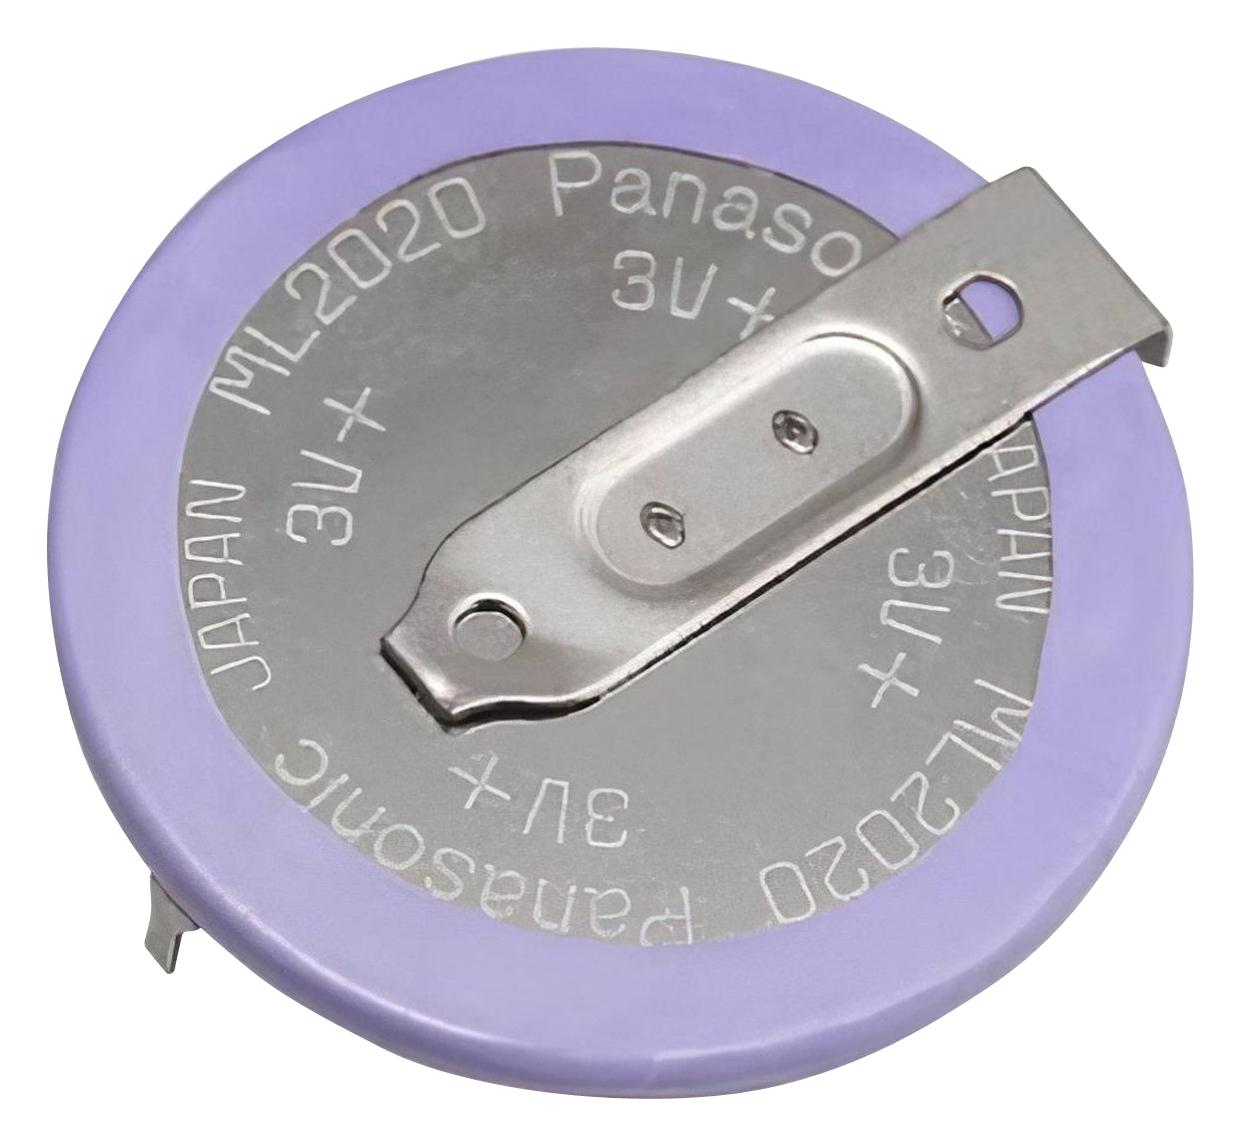
\includegraphics[width=0.5\marginparwidth]{figures/results_coin/panasonic_ML2020_photo.jpg}
  \captionof{figure}{Panasonic ML2020 coin cell format battery used to test long-term cycling with dynamic impedance spectroscopy.}
  \label{fig:coin cell}
}
Furthermore, I demonstrate that the presence of a multi-sine perturbation continuously applied during the dynamic impedance spectroscopy test does not affect cell aging.

% Summary of experiments
This study comprises the following measurements:
\begin{table}[h]
\begin{tabular}{ccc}
\toprule
Measurement type & Number of cells & Number of cycles  \\
\midrule
DEIS during CC-CV & 9 & 30\\
Traditional CC-CV& 12& 22--30\\
EIS during interrupted CC-CV & 3& 1 \\
\bottomrule
\end{tabular}
\end{table}

\section{Experimentals}

\subsection{Cell choice}
% Cell chemistry and implications
For this research, I acquired a set of identical Panasonic ML2020 coin cell batteries containing manganese dioxide (MnO$_2$) as the positive electrode and a lithium--aluminum alloy as the negative electrode. 
The lithium content is approximately 0.02~g. 
These cells utilize an electrolyte solution composed of 1,2-dimethoxyethane and ethylene glycol dimethyl ether (EGDME) combined with an unspecified lithium salt.

According to manufacturer specifications, these batteries have a nominal capacity of 45~mAh and are designed to operate within a voltage window of 1--3~V, with a recommended charging current of 100~$\mu$A. 

The cells exhibit relatively slow kinetics compared to NMC/graphite systems due to the viscosity of the electrolyte, and they experience rapid capacity fade---a characteristic of low-power designs at modest C-rates. 
They are designed as buffers for low-power electronics; thus, a viscous solvent is used as the electrolyte to reduce self-discharge.
When cycling at a C-rate of C/10, the cells degrade rapidly, reaching end-of-life in approximately 22 cycles, with short-circuits often observed. 
I attribute this to lithium plating in dendritic form.

These limitations are actually favorable for rapidly iterating optimizations of the set-up.
The use of commercial cells ensures reproducibility for validation of the method. 

\subsection{Dynamic impedance spectroscopy measurements}

\subsubsection{Setup description}
% \marginpar{
%   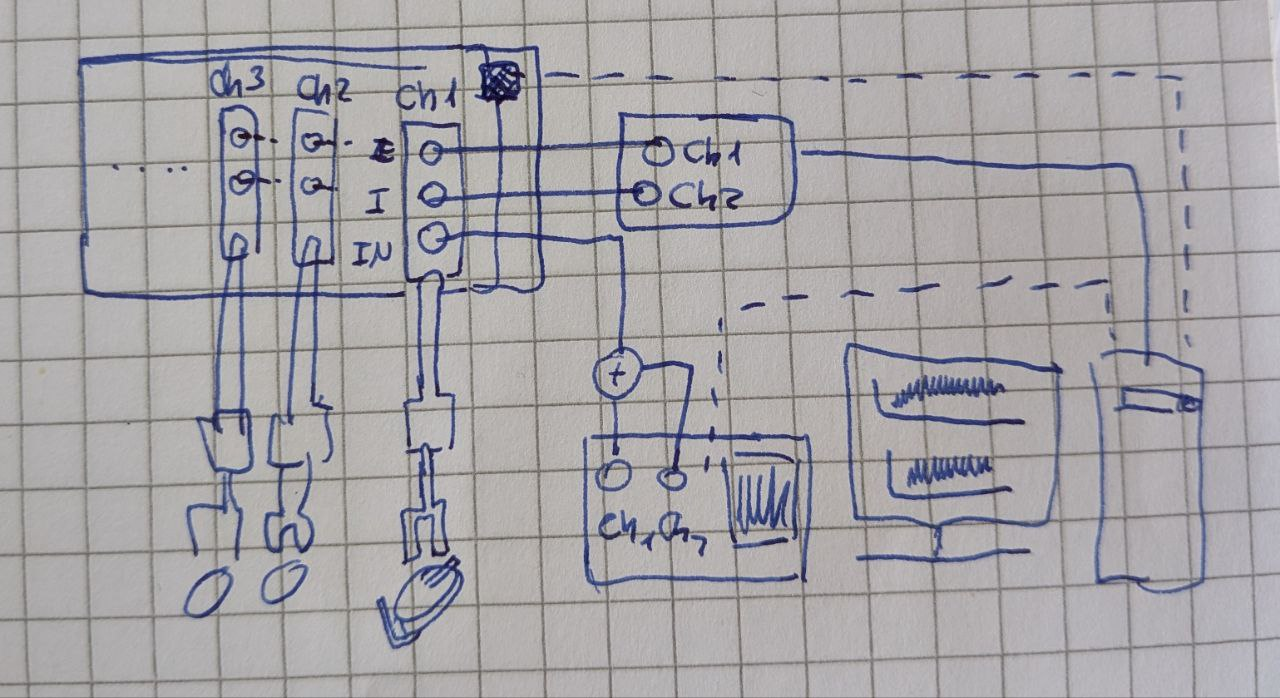
\includegraphics[width = 0.8\marginparwidth]{figures/results_coin/sketch_DEIS_setup_new.jpg}
%   \label{fig:DEIS setup coins}
% }
I conducted the measurements of this chapter using the setup configured for broadband multi-sine waves: two channels of the generator apply two multi-sine excitations covering a total of 7 frequency decades, and the computer processes the streamed data from the oscilloscope in real time as described in Section~\ref{On-line computation}. 
Three of the six channels of the BioLogic SP-300 potentiostat were measured simultaneously thanks to the multi-threading capability of the software \verb|EIStools|. 
% The connection of the instruments is shown in Figure~\ref{fig:DEIS setup coins}.

\subsubsection{Multi-sine design}
The multi-sine waveform excitation contains 49 frequency components in the range 10~mHz--100~kHz, generated at 250~kSa/s, thus one period is of 100~s. 
The total waveform is split into two parts as described in Section~\ref{sec:multisine split} to work around the memory limitation of one generator channel. 
The amplitude of the multi-sine was optimized from a previous experiment as described in Section~\ref{sec:amplitude optim}. 

\subsubsection{Applied drift}
The potentiostat applies a constant current--constant voltage (CC-CV) sequence with an upper voltage limit of 3~V during charge and the same value for the constant voltage step with a lower current limit of 1~mA. The lower voltage limit for discharge was 1~V. The applied current was 4.5~mA, equivalent to a C-rate of C/10. Because of the multi-sine perturbation, the limits are checked during the online computation algorithm as the average value of the data block (as described in Section \ref{sec:software_limits}). The cells are cycled for 30 cycles continuously or until reaching end-of-life. 

The voltage and current signals are sampled with a two-channel PicoScope 4000 series at a sampling rate of 500 kSa/s.

After the experiment, the automated software returns the impedance of the high frequencies (10 Hz--100 kHz) computed online using the STFT method and the voltage and current signals from the cells at the reduced sampling rate of 50 Sa/s. The signals contain the lowest 21 frequency components, ranging from 10 mHz to approximately 8 Hz.

To illustrate the output of the online computation and data-reduction pipeline, Figure \ref{fig:raw_multifrequency_coin} shows the reconstructed voltage and current signals after filtering and downsampling as it is saved in the computer storage after the acquisition step.
These signals retain the low-frequency components while discarding high-frequency content already processed online.

\begin{figure}[h]
  \centering
  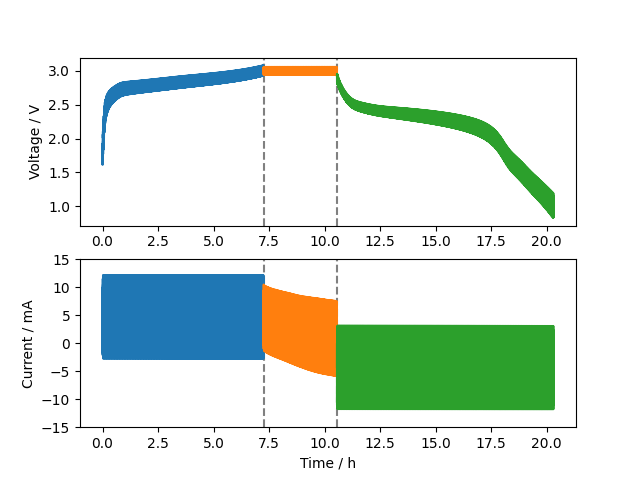
\includegraphics[width = \textwidth]{figures/results_coin/raw_data_multifrequency.png}
  \caption{Voltage and current signals sampled at 50 Sa/s after online computation and downsampling.
  The signals contain the low-frequency components (10mHz--8Hz) of the original broadband excitation, which are used for off-line DMFA estimation of the impedance and reconstruction of the electrochemical drift.}
  \label{fig:raw_multifrequency_coin}
\end{figure}

The impedance of the lower frequency band and the drift are estimated using the DMFA with a filter bandwidth of 0.01 Hz, which yields a time resolution of 100 s, equal to one period of the multi-sine and the signal block used in the online computation. The total impedance spectrum is the concatenation of the parts computed with STFT and DMFA and reported in Figure \ref{fig:dmfa_impedance_coin}.

\begin{widefigure}[!h]
  \centering
  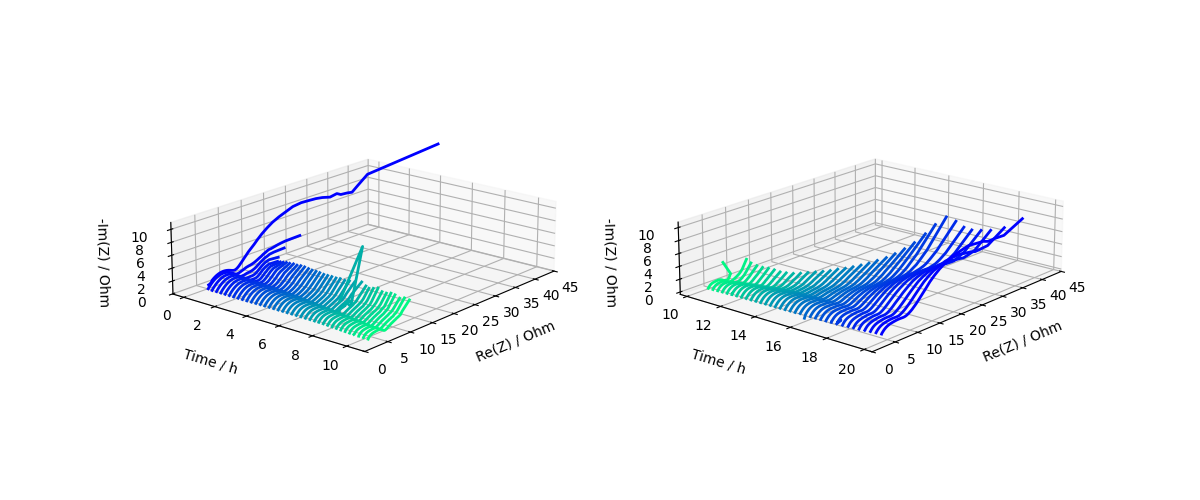
\includegraphics[width = \linewidth]{figures/results_coin/dmfa_impedance_result.png}
  \caption{Impedance of charge and discharge estimated with DMFA and online STFT combined. One spectrum per 10 cycles is plotted; the first 2 plots are discarded.}
  \label{fig:dmfa_impedance_coin}
\end{widefigure}

The effectiveness of the DMFA in separating the slow electrochemical drift from the superimposed multi-sine excitation is illustrated in Figure \ref{fig:dmfa_drift_coin}.

\begin{figure}[h]
  \centering
  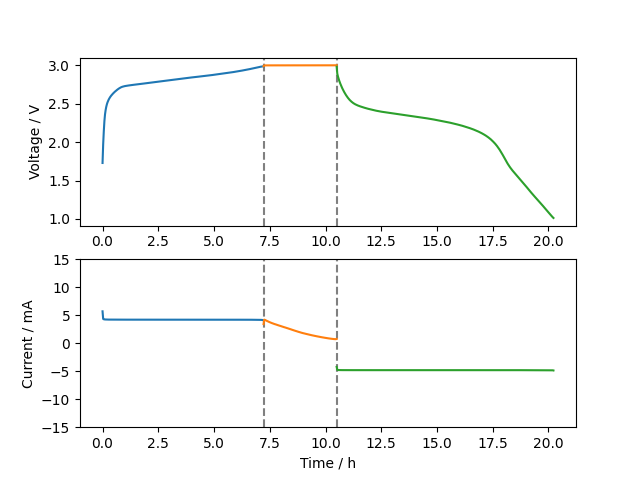
\includegraphics[width = \textwidth]{figures/results_coin/dmfa_drifts_result.png}
  \caption{Drift reconstructed using the DMFA from the downsampled voltage and current signals. The y-axis scale is kept the same as in Figure \ref{fig:raw_multifrequency_coin} for comparison.}
  \label{fig:dmfa_drift_coin}
\end{figure}

\subsection{Impedance analysis}
\subsubsection{General transfer function model}
A battery contains at least two principal interfaces (positive and negative electrodes), whose impedances are connected in series in an equivalent circuit model.
This makes it challenging to develop a physical model that effectivelly describe the system without overparametrize.

% In this work, I approached the identification problem as a black-box and used a rational polynomial function for fitting through complex nonlinear least-squares:
% \begin{equation}
%   Z (\sqrt{j\omega})= \frac{a_0 + a_1(j\omega)^{-1/2}+\cdots+a_n(j\omega)^{-n/2}}{1 + b_1(j\omega)^{-1/2}+\cdots+b_n(j\omega)^{-n/2}}.
% \end{equation}
% Setting $b_0 = 1$ prevents the function from diverging.


Instead of attempting to identify its physical parameters with a physical model (referred as a white-box model) it is equally interesting to identigy the system with a matematical model (referred as a black-box model). 
Thanks to the continous instantaneous impedance spectra generate with dynamic impedance spectroscopy, the time varaition of the mathematical model's parameters remains informative for the purpose of control and prediction. 

In this context of system identification, the battery is considered a generic linear and time-invariant system, hence the input $u(t)$ and the output $y(t)$ of a system are connected by the linear ordinary differential equation
\begin{equation}
    \sum_{N} a_n \frac{\text{d}^ny(t0)}{dt} = \sum_{M} b_m \frac{\text{d}^my(t0)}{dt}.
\end{equation}
As discussed in Section \ref{sec:laplace}, differential equation can be solved by applying the Laplace transform, which yields
\begin{equation}
    \sum_{N} a_n s^n Y(s) = \sum_{M} b_m s^m U(s),
\end{equation}
and so the transfer function for the system is given by
\begin{equation}
    G(s) = \frac{Y(s)}{U(s)}=\frac{\sum_{N} a_n s^n}{\sum_{M} b_m s^m}.
\end{equation}
This equation for the transfer function is the same of Equation \ref{eq:transfer function dy sys} from section \ref{sec:transfer function def diff equations} (p. \pageref{sec:transfer function def diff equations}).

The Laplace variable $s$ for the case of impedance is simplified to $s = j\omega$, but since the system is electrochemical, the homogeneous differential equations describing diffusion are semi-integer \cite{oldhamFractionalDifferentialEquations2010} and lead to solutions as functions of $\sqrt{j\omega}$.
Therfore for electrochemical systems the generic transfer function has the form:
\begin{equation}
    G(\sqrt{j\omega}) = \frac{\sum_{N} a_n (\sqrt{j\omega})^n}{\sum_{M} b_m (\sqrt{j\omega})^m}.
    \label{eq:general rational polynomial}
\end{equation}

In this work, I used such a rational polynomial function of order $n=m$ as a measurement model to fit impedance data.
The concept is not new \cite{zoltowskiNontraditionalApproachMeasurement2005,gheemTheoreticalApproachModelling2008a,liModelReductionFractional2024}, but it is the first time this model has been used for instantaneous impedance of time-varying systems.
Polynomial functions can flexibly fit impedance with any complex shapes and also have the advantage of working as a test for the linear Kramers-Kronig relations \cite{sadkowskiCNLSFitsKramers2004}.

\subsubsection{Regression procedure}

A fundamental procedure for the regression of rational polynomial function is to add L1 regularization to the objective function, also called LASSO (\emph{least absolute shrinkage and selection operator}).
In practice, the objective function to minimize is
\begin{equation}
  obj = \sum_n r_n^2 + \lambda ||\mathbf{\theta}||_1,
\end{equation}
where $r_n^2$ is the weighted complexed squared residual of the n-th point of the spectra as described in Section \ref{sec:fitting-sys-id}, $\mathbf{\theta}$ is the parameters array, and $\lambda$ is a penalty factor that controls the regularization strength.
Regularization is important because rational function parameters can grow unnecessarily large and be compensated by parameters in the denominator.
The choice of penalty factor is arbitrary, and I found that values as small as $1 \times 10^{-12}$ is sufficient.
Removing the regularization terms makes the optimization procedure ineffective (parameters diverge) or causes the solver to fail.


Before fitting, I removed the first three and last two spectra from the dataset, as well as the first three and last frequency points (remaining range: 30~mHz--42~kHz).

In least squares objective function introduced in Section \ref{sec:fitting-sys-id} each frequency component residue is weighted by a factor equal to the experimental error.
The error in a frequency response function increases with the lowering of the frequency.
Orazem et al.\cite{orazemEIS} originally proposed to use the inverse of the impedance modulus as weighting factor, but I found that using the square root of the modulus is more effective in this case. It weights the middle-to-high frequency range more heavily, allowing the model to fit the impedance's features better.

A better strategy would be to estimate the error from error propagation rules through elementary mathematical operations, as described in Reference \cite{chukwuStatisticalAnalysisMeasurement2022} did for admittance data estimated via DMFA.
Unfortunately, I was unable to replicate his derivation for my impedance data.
Furthermore, error propagation for the FFT impedance method is not available in the literature and must be derived from first principles.

For the optimization, I adopted a classical derivative-based approach (trust region reflective method) as implemented in the Python package \verb|LMFIT| \cite{newville_2014_11813} to solve such minimization problems.
I first fited the spectrum at the middle of the dataset using random initial parameters (seed 42) and then used the optimized parameters as the starting points for the first spectrum of the dataset. Subsequently, I proceed passing optimized parameters as initial points for the next fitting.

% Regarding the order of the rational polynomial, I chose the same order for numerator and denominator and found that 7 was the minimum order needed to represent all features with a small error.

The difficulty in fitting dynamic impedance data is identifying one set of values for polynomial order, regularization penalty factor, and least-squares weighting factor that work effectively across all electrochemical techniques in the experiment, all cycles, and are general enough to apply to multiple cells.

\subsection{Classical electrochemical test}
I performed cycling experiments using the same constant current--constant voltage protocol on a BioLogic battery cycler with 12 cells from new to aged condition to compare degradation with and without multi-sine excitation.

I also prepared an experiment performing classical electrochemical impedance spectroscopy at fixed states of charge. For this purpose, I created an experiment sequence that interrupts the cycling protocol every 10\% of the nominal capacity and includes a 1~h rest before impedance measurement in the frequency range 10~mHz--20~kHz (8~points/decade).


\section{DEIS results}

% Geometrical features across SoC (semicircles, diffusion tail, ohmic resistance) 
% and their evolution with SoH

% First cycle behavior and conditioning affects impedance

% Cell-to-cell variability and outliers

\subsection{Impedance at different battery states}

Continuous impedance acquisition provides a complete view of battery interface resistance at any state of charge and state of health. Figures~\ref{fig:deis_aging_charge} and~\ref{fig:deis_aging_discharge} show this information for charge (including the potentiostatic portion) and discharge. I compared the impedance at four states of health corresponding to the beginning, midpoint, just before the 80\% threshold of first-cycle capacity, and after it. 
It can be observed at least two consecutive semicircles and a diffusive tail. At lower states of charge, represented in red in the colored scale, a third semicircle appears, shifting the diffusion to lower frequencies.
Another observation is the change in ohmic drop resistance with state of charge.
The evolution of the impedance spectrum with battery aging during charge is summarized in Figure~\ref{fig:deis_aging_charge}.

\begin{widefigure} [h]
  \centering
  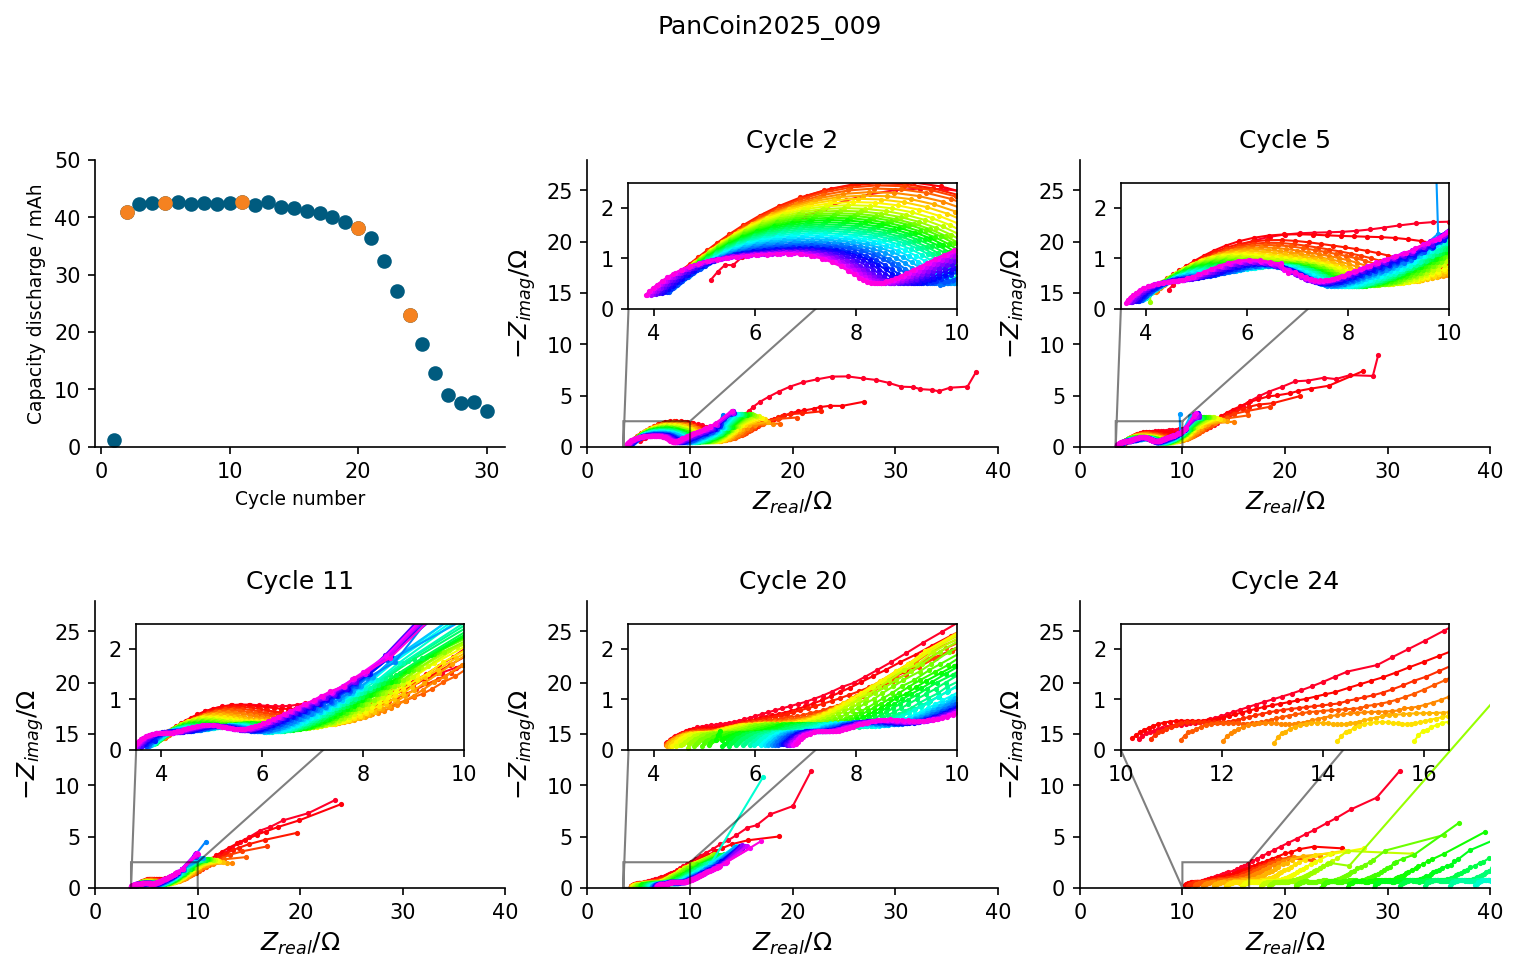
\includegraphics[width = \linewidth]{figures/results_coin/PanCoin2025_009_DEIS_charge_aging_mosaic.png}
  \caption{Dynamic impedance spectra during charge at selected states of health.
  Spectra are shown for four aging stages: beginning of life, mid-life, just before the 80\% capacity threshold, and after crossing it.
  Color coding indicates state of charge.}
  \label{fig:deis_aging_charge}
\end{widefigure}

A corresponding representation for discharge is reported in Figure~\ref{fig:deis_aging_discharge}.

\begin{widefigure} [!h]
  \centering
  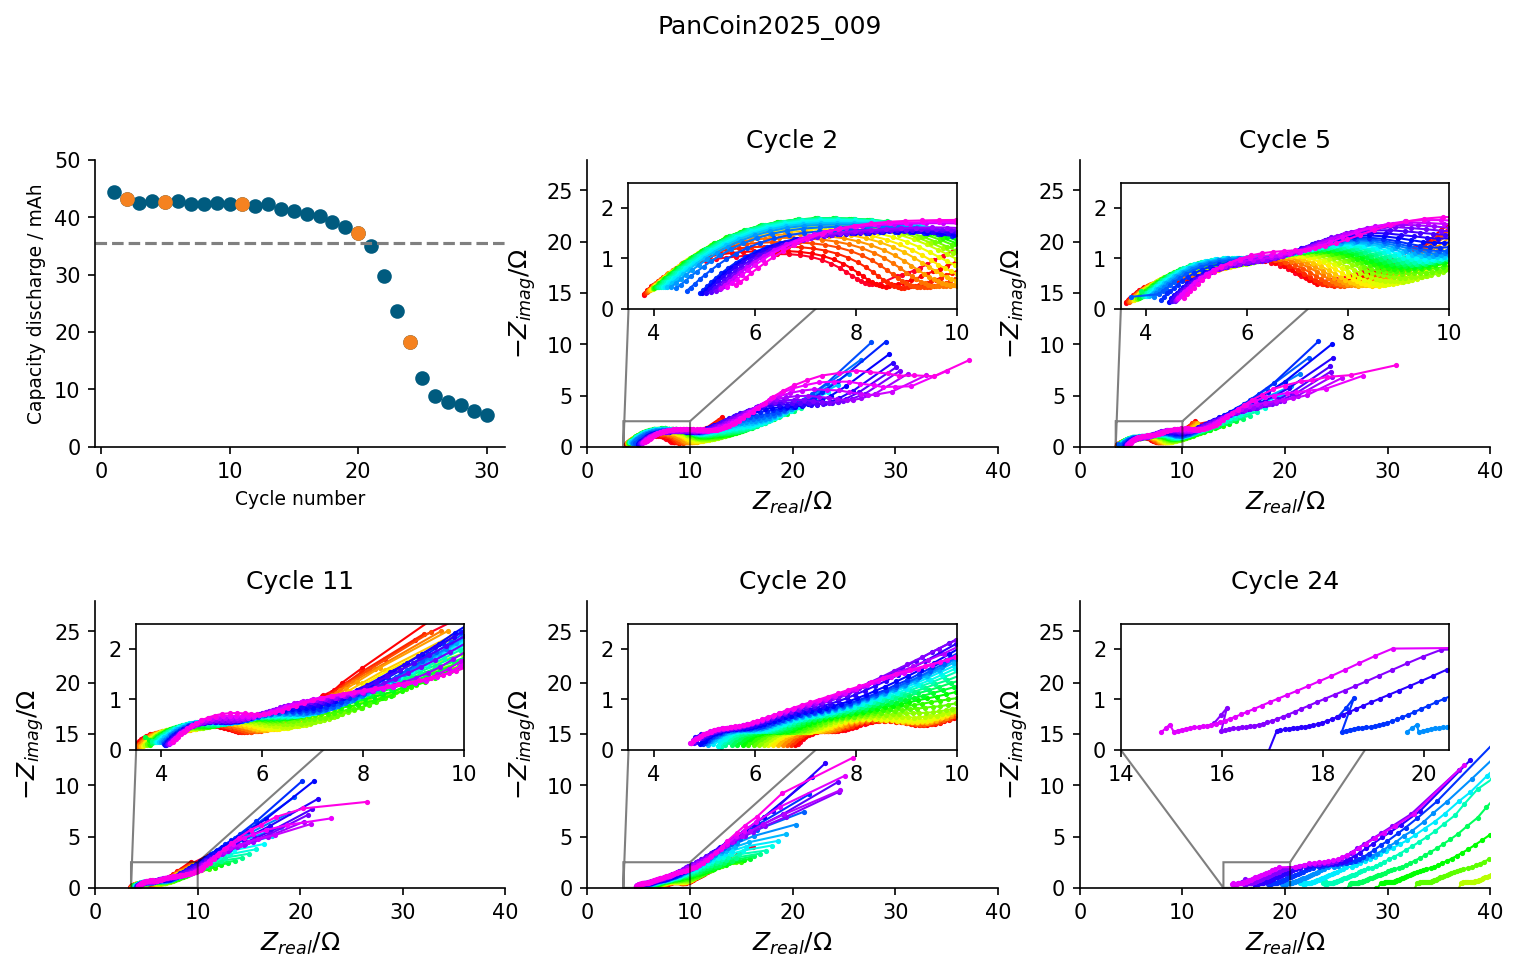
\includegraphics[width = \linewidth]{figures/results_coin/PanCoin2025_009_DEIS_discharge_aging_mosaic.png}
  \caption{Dynamic impedance spectra during discharge at the same aging stages as Figure~\ref{fig:deis_aging_charge}.
  The appearance and shift of multiple semicircles and diffusive features reflect changes in interfacial and transport processes with aging.}
  \label{fig:deis_aging_discharge}
\end{widefigure}

The cell is provided from the manifacturer at 2.75~V, so in the first cycle of the measurement, the cell voltage quickly reaches the charging limit and then precedes the discharge as shown in Figure~\ref{fig:first_cycle_coin}. 
The impedance of the first cycle is reported in Figure \ref{fig:impedance_first_cycle_coin}
% This is probably due to the state of the solid electrolyte interphase (SEI). 
% After the fir charge the SEI is damaged and freshly reformed in the next discharge. 
% I also expect some lithium deposition alongside the alloying with aluminum during the negative electrode reduction that increase the surface area exposed to the electrolyte yielding to further SEI formation.
% Looking at both impedance magnitudes, though, a reduction is noted for the cycles after the second.
% This might be connected to a thinner SEI layer.

\begin{figure} [!h]
  \centering
  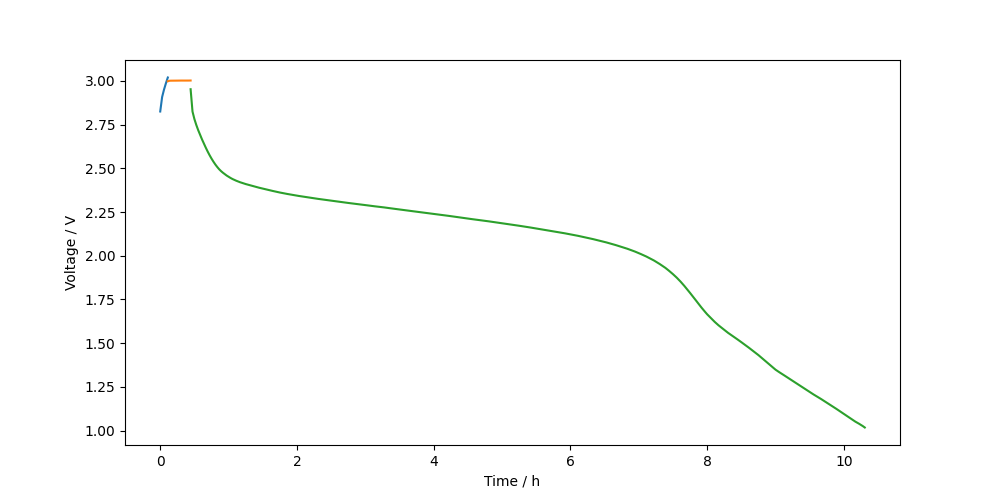
\includegraphics[width = \textwidth]{figures/results_coin/Voltage_dmfa_first_cycle_cell009.png}
  \caption{Voltage profile of the first charge--discharge cycle.
  The cell reaches the upper voltage limit early during the first charge, indicating a conditioning process that differs from subsequent cycles.}
  \label{fig:first_cycle_coin}
\end{figure}


\begin{figure} [!h]
  \centering
  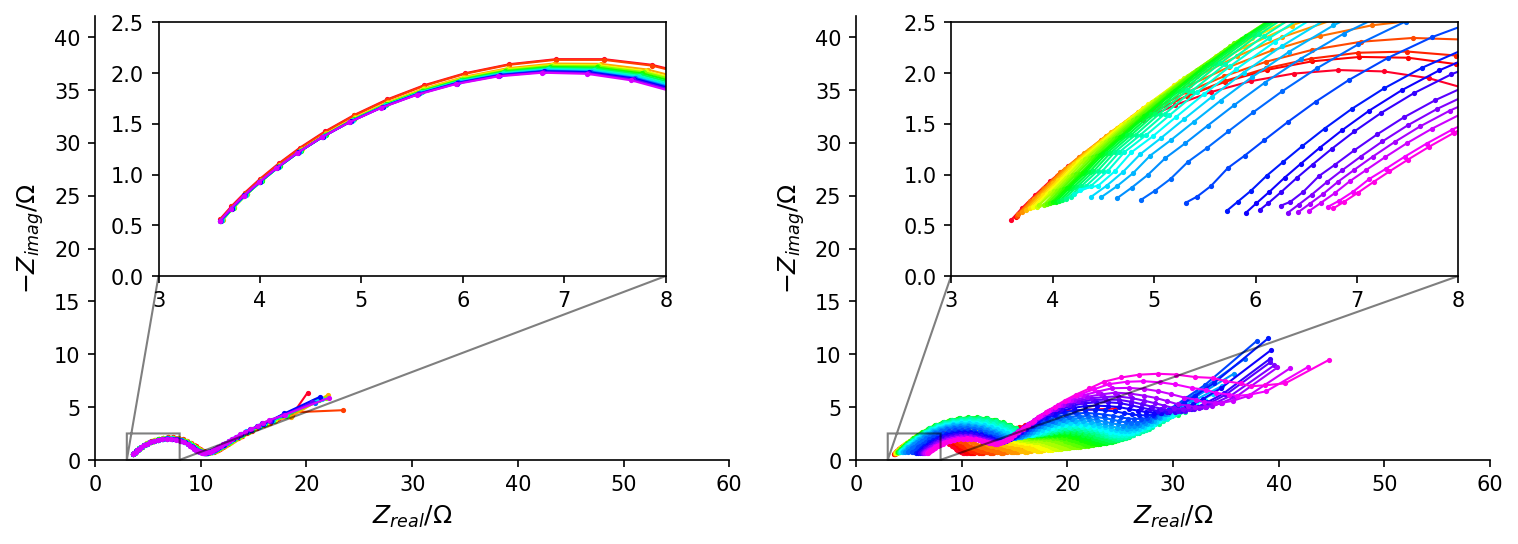
\includegraphics[width = \textwidth]{figures/results_coin/PanCoin2025_009_DEIS_first_cycle.png}
  \caption{Impedance spectra during the first cycle.
  Left: all charge spectra; right: discharge spectra with one spectrum every ten cycles.
  Both magnitude and shape differ markedly from later cycles, indicating transient interfacial processes during initial conditioning.}
  \label{fig:impedance_first_cycle_coin}
\end{figure}

All behaviors observed here are reproduced in the other 8 cells of the set, including the higher impedance in the first discharge. Detailed results are reported in the Appendix. 
The reproducibility of the dynamic impedance measurements across nominally identical cells is assessed in Figure~\ref{fig:eis_dynamic_variability}.

\begin{widefigure} [!h]
  \centering
  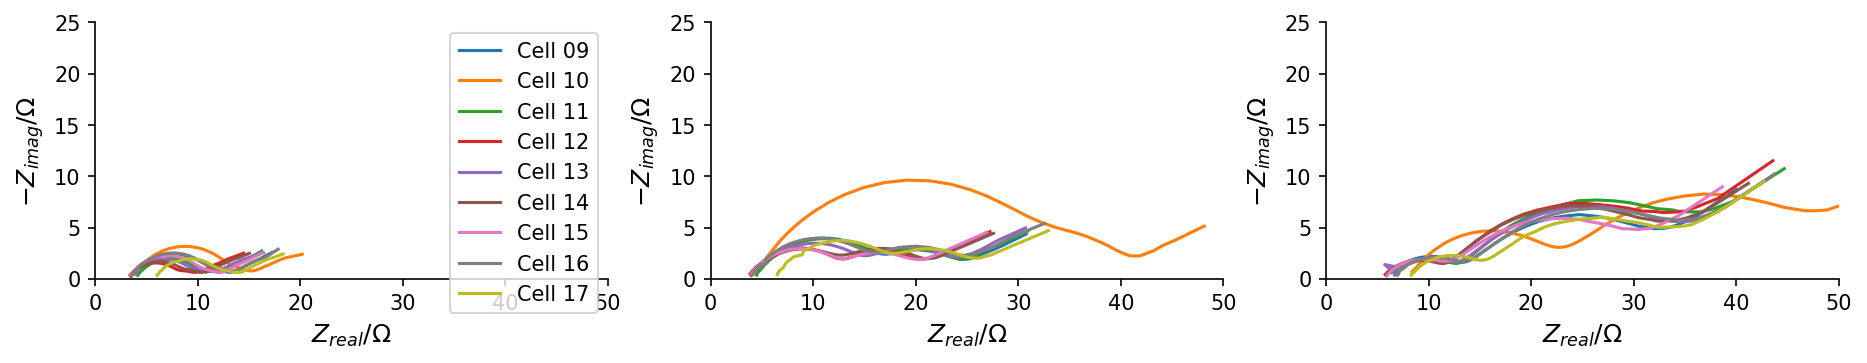
\includegraphics[width = \linewidth]{figures/results_coin/eiS_dynamic_variability.png}
  \caption{Dynamic impedance variability across nine cells at 90\%, 50\%, and 10\% state of charge during the second discharge half-cycle.
  While overall spectral features are consistent, variations in magnitude and ohmic resistance reflect manufacturing variability.}
  \label{fig:eis_dynamic_variability}
\end{widefigure}

As with any production process, cells do not respond identically but show similar behavior. One can notice impedance magnitude variations for Cell~10 and variations in the ohmic drop, which is notably higher in Cell~17 than in the others.

% Comparing complex impedance qualitatively in the complex plane across many cells in two dimensions (state of charge and state of health) is challenging. A better approach is to fit the data with a model and compare the fittedcoefficients. Not only are they fewer than the number of impedance points (10--15 versus 50), but they are also real-valued.

\subsection{Effect of the multi-sine on aging}
To assess whether continuous multi-sine excitation influences degradation, capacity retention is compared statistically in Figure \ref{fig:aging_comp}.

\begin{figure} [!h]
  \centering
  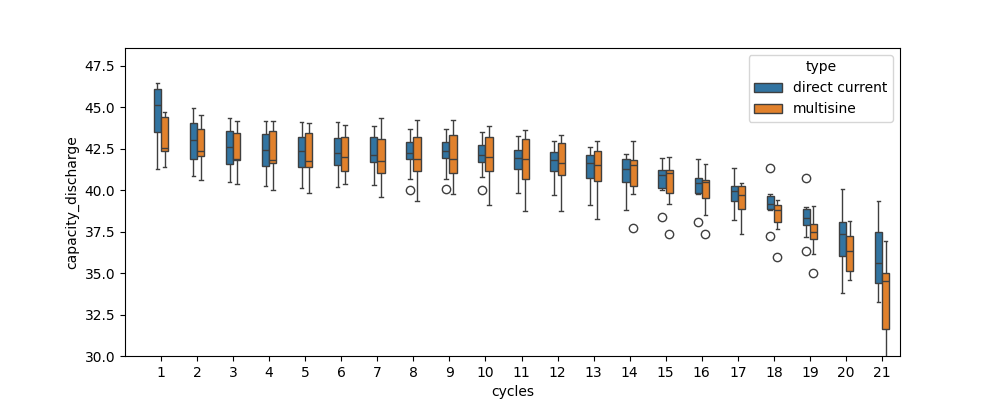
\includegraphics[width = \textwidth]{figures/results_coin/Boxplot_aging.png}
  \caption{Comparison of discharge capacity retention for cells cycled with DC-only excitation and DC with superimposed multi-sine perturbation.
  Boxplots summarize the distribution across 12 DC-only cells and 9 DEIS cells, showing no statistically significant difference under the tested conditions.}
  \label{fig:aging_comp}
\end{figure}

The reduce y-axis scale highlights the marginal differences between the two datasets, therefore I conclude that the multi-sine is not impacting the cycling performance and can be applied continously for system identification; at least for this small cells at low C-rate.

\subsection{Effect of the drift on the impedance}
Static impedance measured at different states of charge also shows good consistency. Figure~\ref{fig:eis_static_variability} reports data from three cells at the same states of charge as Figure~\ref{fig:eis_dynamic_variability}.
For reference, the variability of stationary impedance measurements obtained during interrupted cycling is shown in Figure \ref{fig:eis_static_variability}.

\begin{widefigure} [!h]
  \centering
  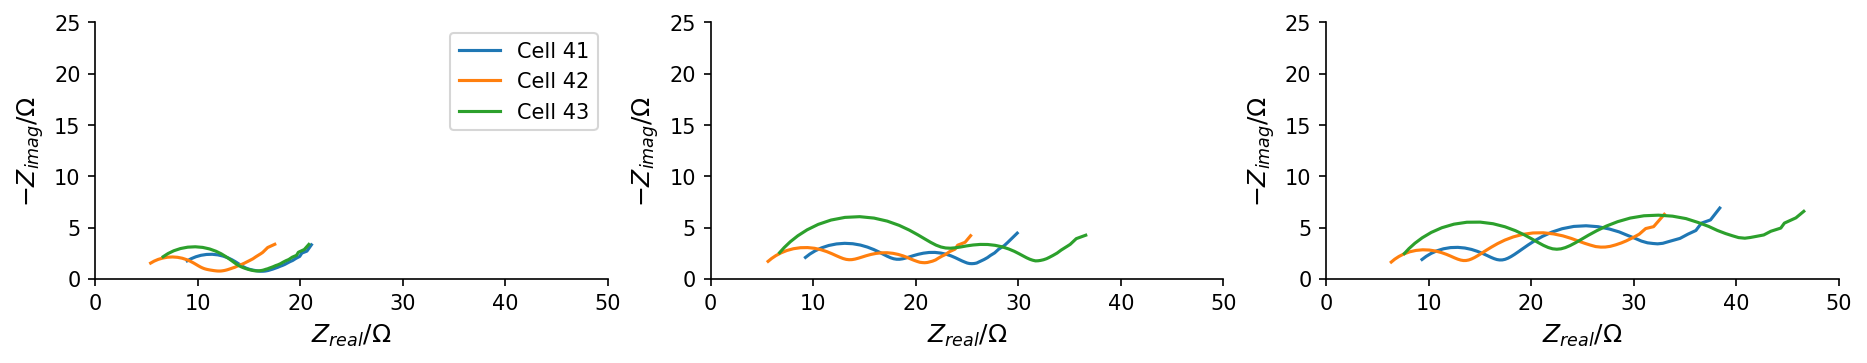
\includegraphics[width = \linewidth]{figures/results_coin/eiS_static_variability.png}
  \caption{Static impedance variability across three cells at selected states of charge.
  Impedance was measured after a 1 h rest at each state of charge using conventional stepped-sine EIS.}
  \label{fig:eis_static_variability}
\end{widefigure}

A direct comparison between static and dynamic impedance measurements is presented in Figure~\ref{fig:eis_static_vs_dynamic}.

\begin{widefigure} [!h]
  \centering
  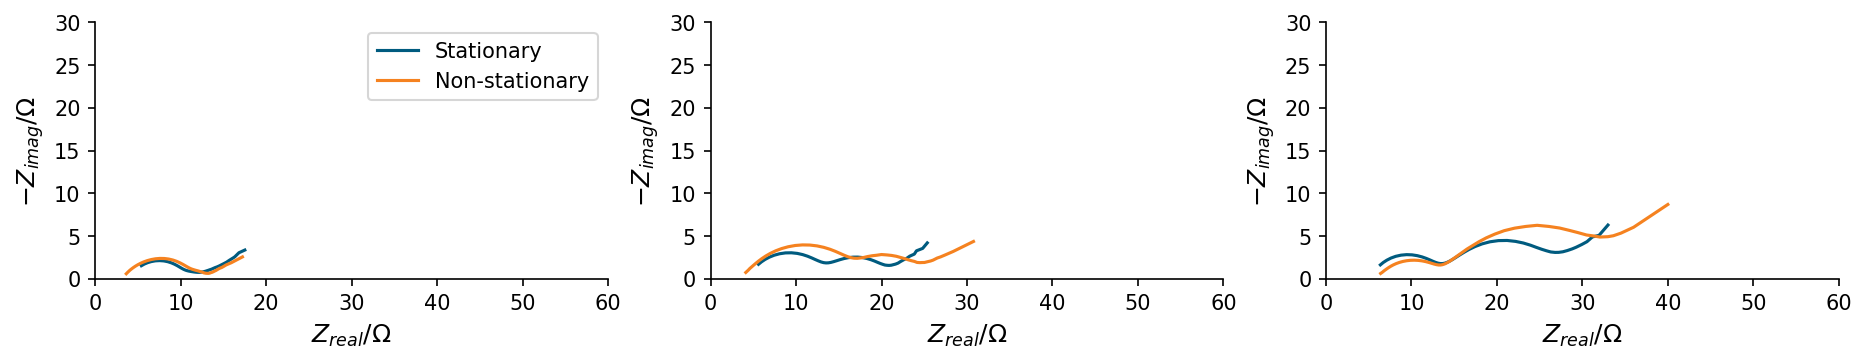
\includegraphics[width = \linewidth]{figures/results_coin/eiS_static_vs_dynamic_soc.png}
  \caption{Comparison of impedance measured under stationary conditions and during non-stationary operation at the same states of charge.
  The close agreement indicates that, at C/10, dynamic impedance measurements capture interfacial properties comparable to equilibrium EIS.}
  \label{fig:eis_static_vs_dynamic}
\end{widefigure}

This result suggests that at such a low C-rate (C/10), the electrode interfaces are in a similar state to the static case, while significantly reducing measurement time.

Comparing the classic and non-stationary measurements, it is clear how much more convenient the multisine perturbation is over the single sine, as reported in Figure \ref{fig:static vs multisine experiment}.
The latter takes around 27 hours to produce 10 spectra, while the multisine-based method outputs 270 spectra in 10 hours.

\begin{figure}[h]
  \centering
  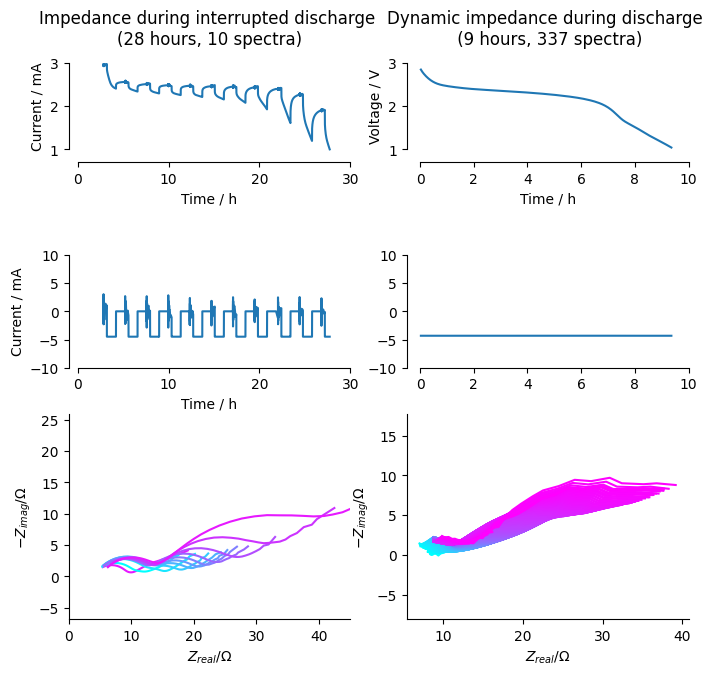
\includegraphics[width = \textwidth]{figures/results_coin/static_vs_dynamic_experiment_discharge_2d.png}
  \caption{Comparison between classic impedance measurement at different equilibrium voltages and a DEIS measurement. The classic experiments takes much longer time and produces fewer spectra. On the right hand side the multi-sine components are filtered out from voltage and current signals and only one over ten of the instantaneous impedances is plotted.}
  \label{fig:static vs multisine experiment}
\end{figure}

\section{Results of fitting}

Evaluating the fitting quality of dynamic impedance data involves multiple assessments: qualitative visualization, magnitude and structure of residuals, and consistency of model parameters across cycles.

In this work, I performed the fitting of rational polynomial functions with orders from 4 to 9. 
From the visual inspection of the fitting results, I arbitrary selected the order 5 because it can represent all the different shapes of instantaneous impedance, as shown in Figure~\ref{fig:results_fitting_coin_cycle5} with the minimum number of parameters. 
The residuals are small for the real part, approximately 1\%, but larger for the imaginary part. The systematic structure of the residuals, especially the pronounced deviations at the highest three frequencies, indicates that the model does not fully reproduce all spectral features of the dataset. 
I believe, this issue is both related to the arbitrary choice of the weighting factors in the least-square objective function and the solver itself.

\begin{figure}[!b]
  \centering
  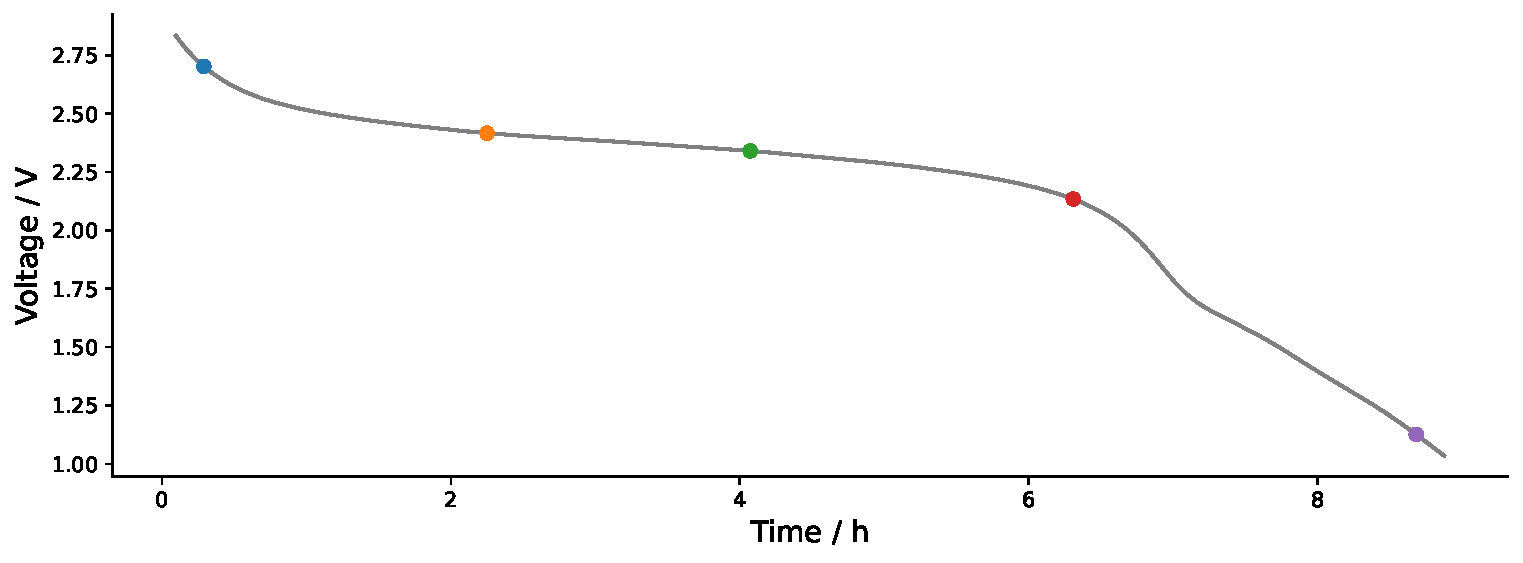
\includegraphics[width=\textwidth]{figures/results_coin/fit_cell009_order5_cycle_5_sequence_4_index_[7, 78, 144, 225, 311].pdf}
  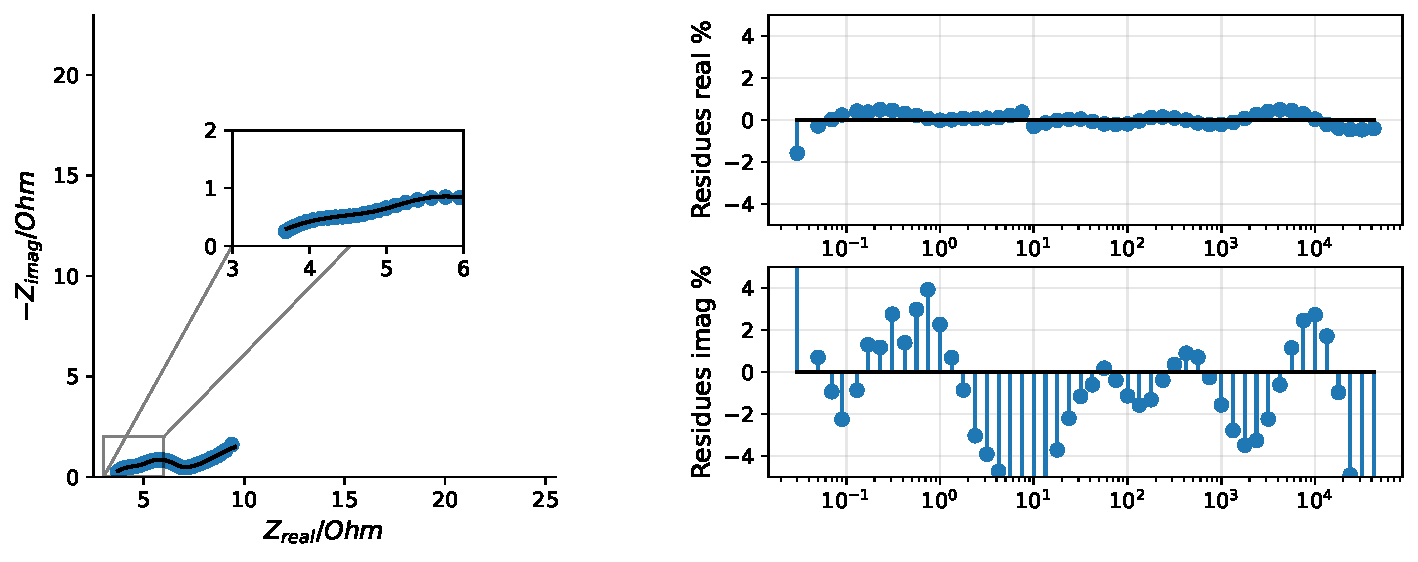
\includegraphics[width=\textwidth]{figures/results_coin/fit_cell009_order5_cycle_5_sequence_4_index_7.pdf}
  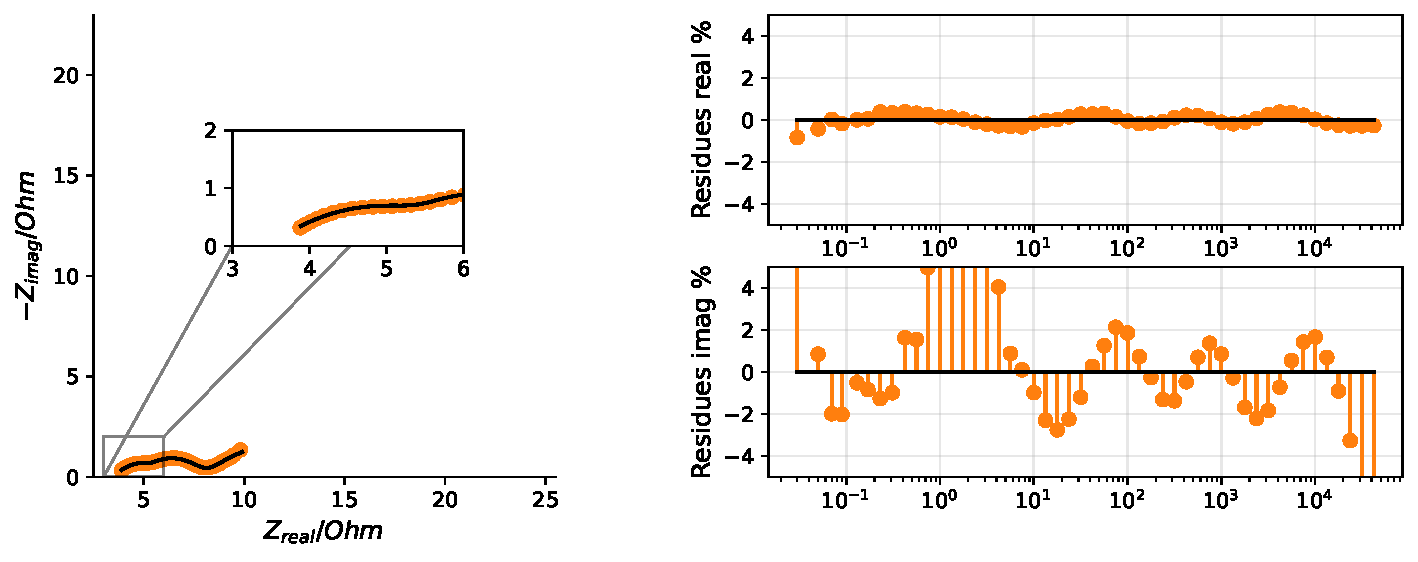
\includegraphics[width=\textwidth]{figures/results_coin/fit_cell009_order5_cycle_5_sequence_4_index_78.pdf}
  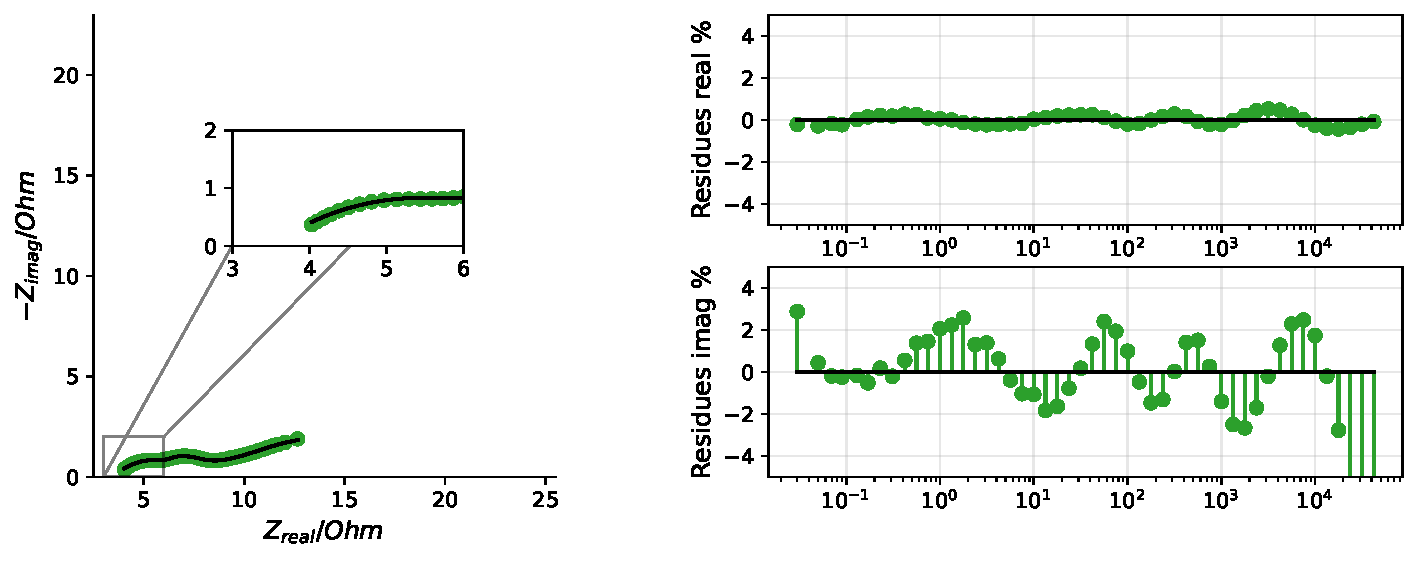
\includegraphics[width=\textwidth]{figures/results_coin/fit_cell009_order5_cycle_5_sequence_4_index_144.pdf}
  \caption{Rational polynomial fitting of dynamic impedance spectra at different states of charge (marked with colors dots) during discharge of cycle 6.
  The figures in the panel after the voltage time series report the impedance data (markers) and fit result (solid black line). Residuals are reported next to each spectrum. The colors of the markers represents the states of charge.}
  \label{fig:results_fitting_coin_cycle5}
\end{figure}
% \clearpage
\begin{figure}[!ht]\ContinuedFloat
  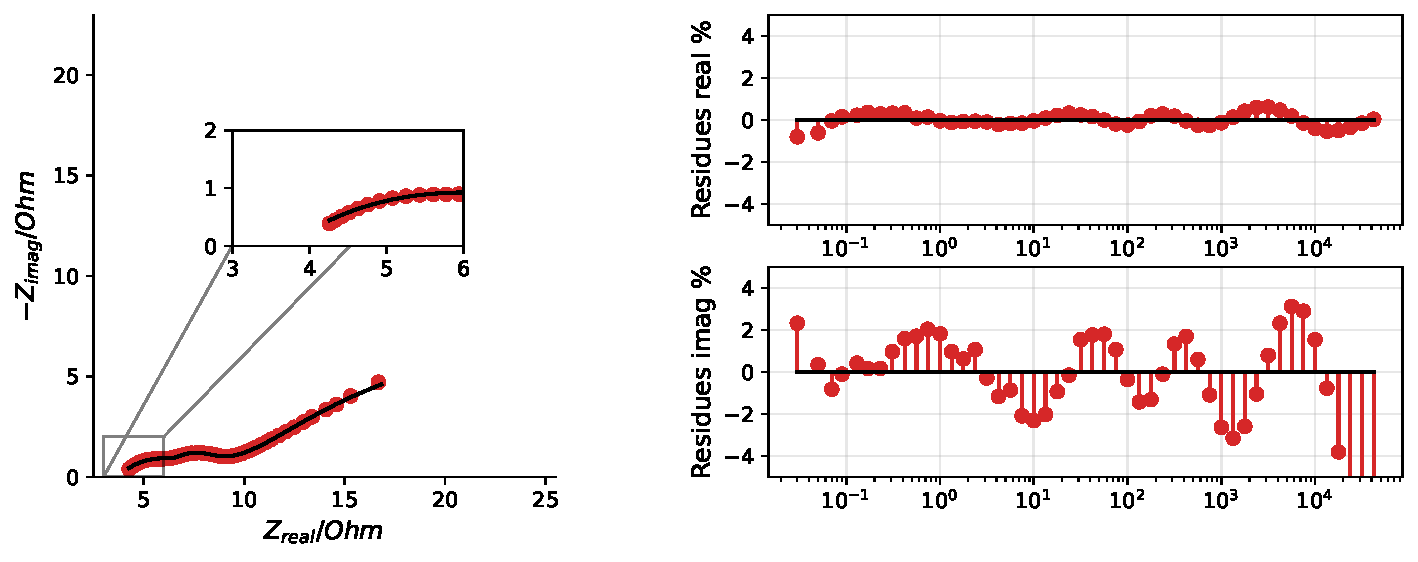
\includegraphics[width=\textwidth]{figures/results_coin/fit_cell009_order5_cycle_5_sequence_4_index_225.pdf}
  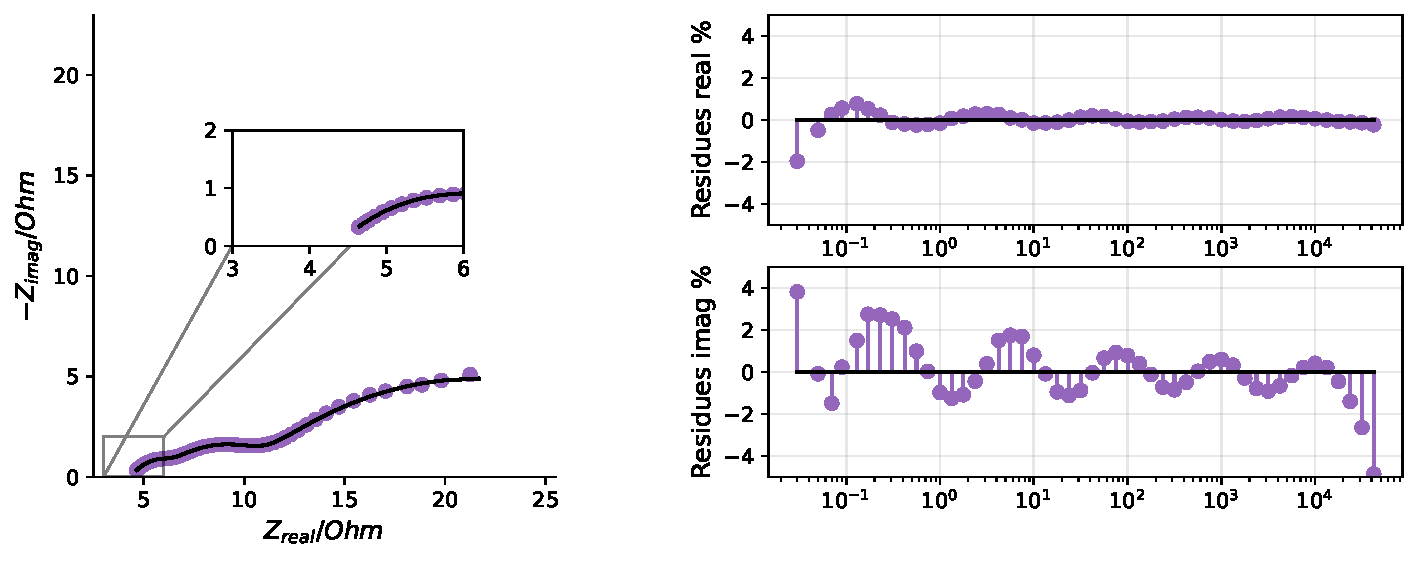
\includegraphics[width=\textwidth]{figures/results_coin/fit_cell009_order5_cycle_5_sequence_4_index_311.pdf}
  \caption[]{Continued}
  % \caption{Rational polynomial fitting of dynamic impedance spectra at different states of charge during discharge of cycle 6.
  % Symbols represent measured impedance; solid lines show the fitted model.
  % Residuals are reported below each spectrum.}
\end{figure}

Despite the small residual magnitudes, their oscillatory behavior persists for polynomial orders up to nine (the highest tested). 
In a well-posed regression problem, residuals are expected to be randomly distributed with magnitude comparable to the measurement variance. 
The persistence of structured oscillations therefore indicates that the limitation is not simply insufficient model order.
The fitting with a smaller order of 4, doesn't lead to a correct representation of the impedance since the model is not capable of resolve the two semicircles at higher frequency. This issue could not be connect with the model structure, but rather the arbitrary weighting factor used in the regression problem.

Despite the criticalities it is interesting to look at the fitting result for order 5 to have an idea of the advantage of parameterization. The fitted parameters vary smoothly across state of charge and state of health although some abrupt magnitude changes are observed when the impedance manifests a new feature (or the features disappears) and the model must adapt to it. 
Representing complex-valued impedance through real-valued model parameters provides a compact description of the spectrum and facilitates subsequent data-driven modeling of cell aging. 
The fitted coefficients can therefore be used as features for machine-learning models to predict state of health.

The evolution of the fitted parameters during cycle~2 across all electrochemical techniques is illustrated in Figure~\ref{fig:fitting_parameters_cycle2}. 
Parameters $a_1$ (orange line) and $a_3$ (red line) exhibit abrupt transitions when a new spectral feature becomes significant: a semicircle emerges at high state of charge and gradually merges into another high-frequency semicircle. 
The parameter jump occurs because the regularized least-squares procedure allow the parameters to increase only when the residual contribution in that region becomes sufficiently large to significantly impact the cost function. 

\begin{figure}[!h]
  \centering
  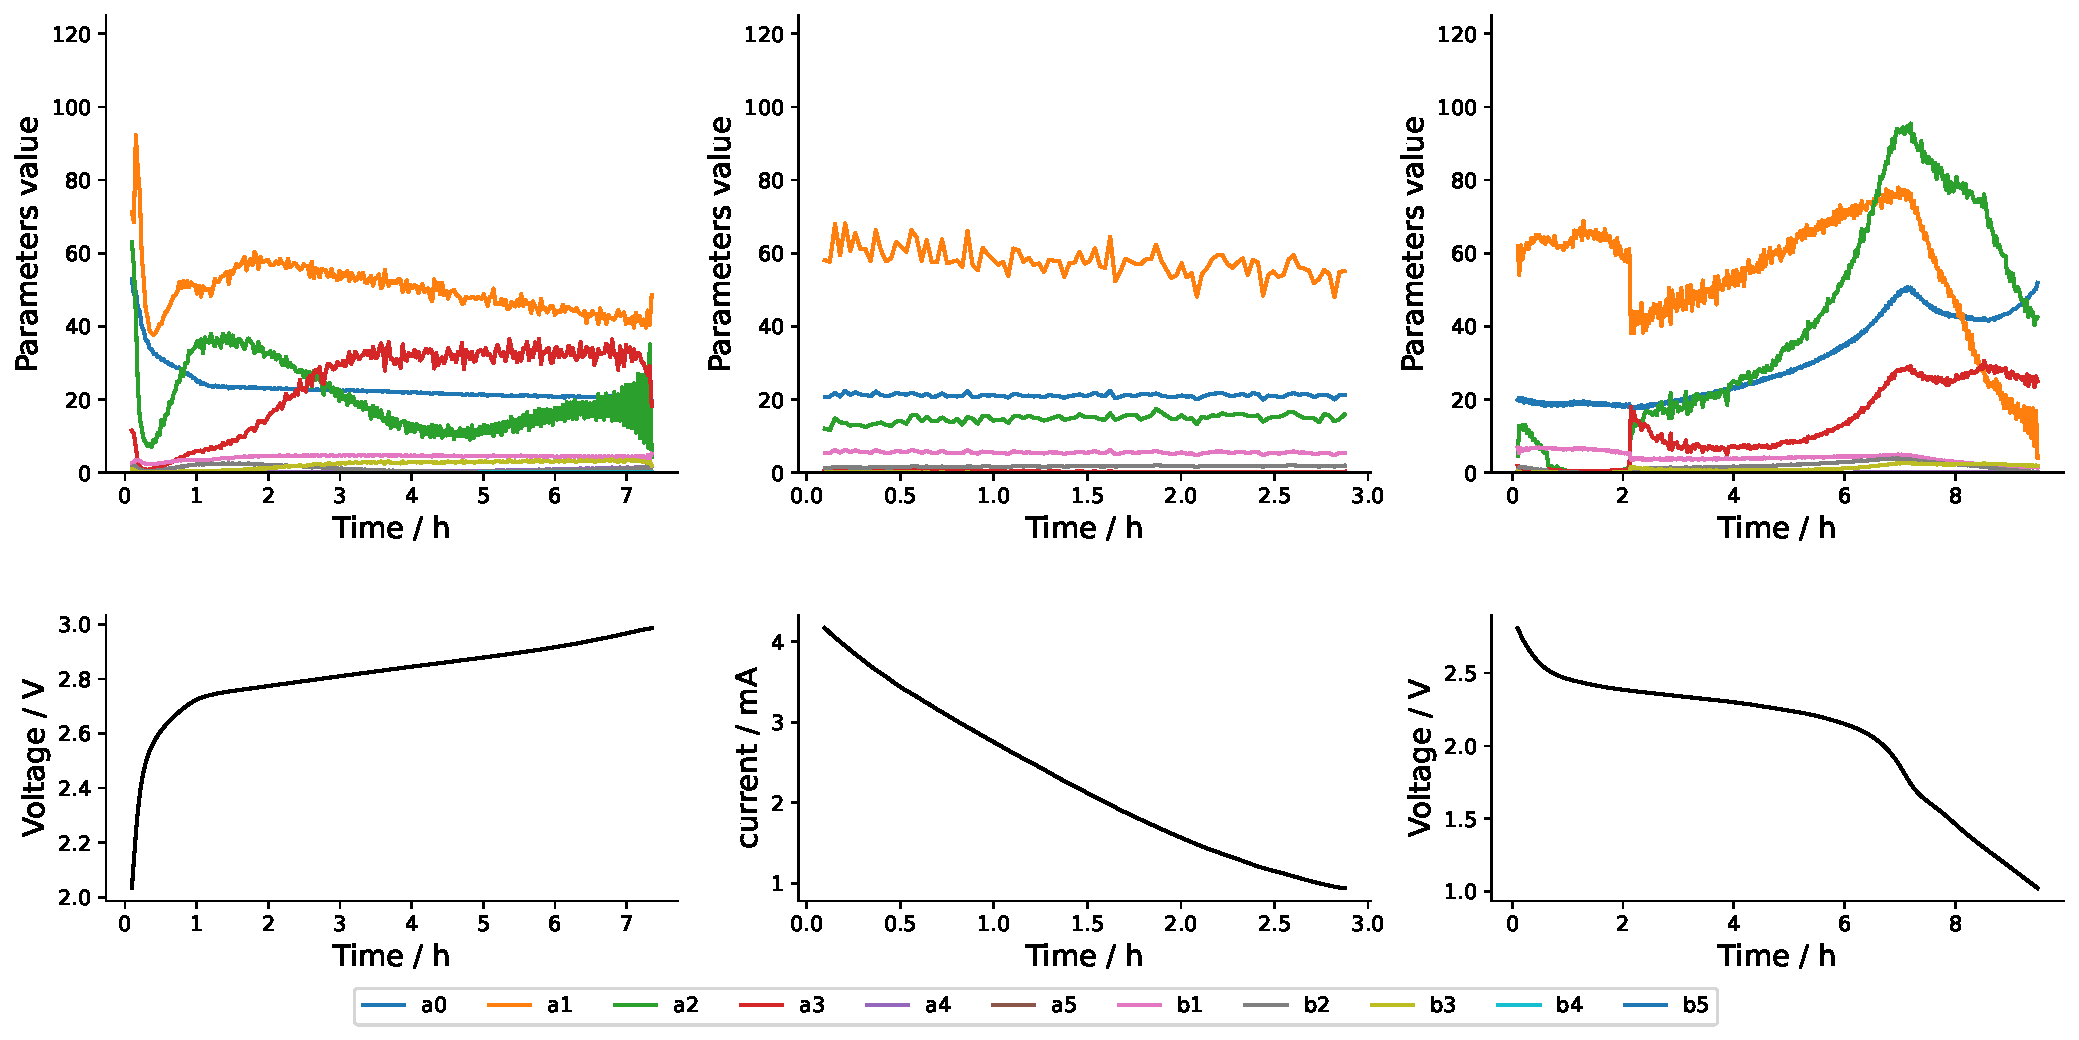
\includegraphics[width = \textwidth]{figures/results_coin/Cell009_fitting_parameters_ouput_order5_cycle1.pdf}
  \caption{Upper row: fitted rational polynomial parameters for all techniques during cycle 2.
  Lower row: corresponding cell voltage and current reconstructed via DMFA.
  Abrupt parameter changes correspond to the emergence of new impedance features.}
  \label{fig:fitting_parameters_cycle2}
\end{figure}

As shown in Figures~\ref{fig:deis_aging_charge} and~\ref{fig:deis_aging_discharge}, after cycle~5 the impedance shape stabilizes, showing two consecutive semicircles followed by a diffusive feature. 
This stabilization is reflected in the corresponding fitted parameters for cycle~5 (Figure~\ref{fig:fitting_parameters_cycle5}) and subsequent cycles (e.g., cycles~10, 15, 20, and 22). 
Parameter magnitudes and trends are largely preserved across cycles and remain mostly continuous within the techniques of the same cycle. 
These observations suggest that, despite their numerical limitations, the fitted parameters capture systematic changes correlated with state of charge and state of health. 
The same qualitative behavior is observed in the results of the other cells.

\begin{figure}[!h]
  \centering
  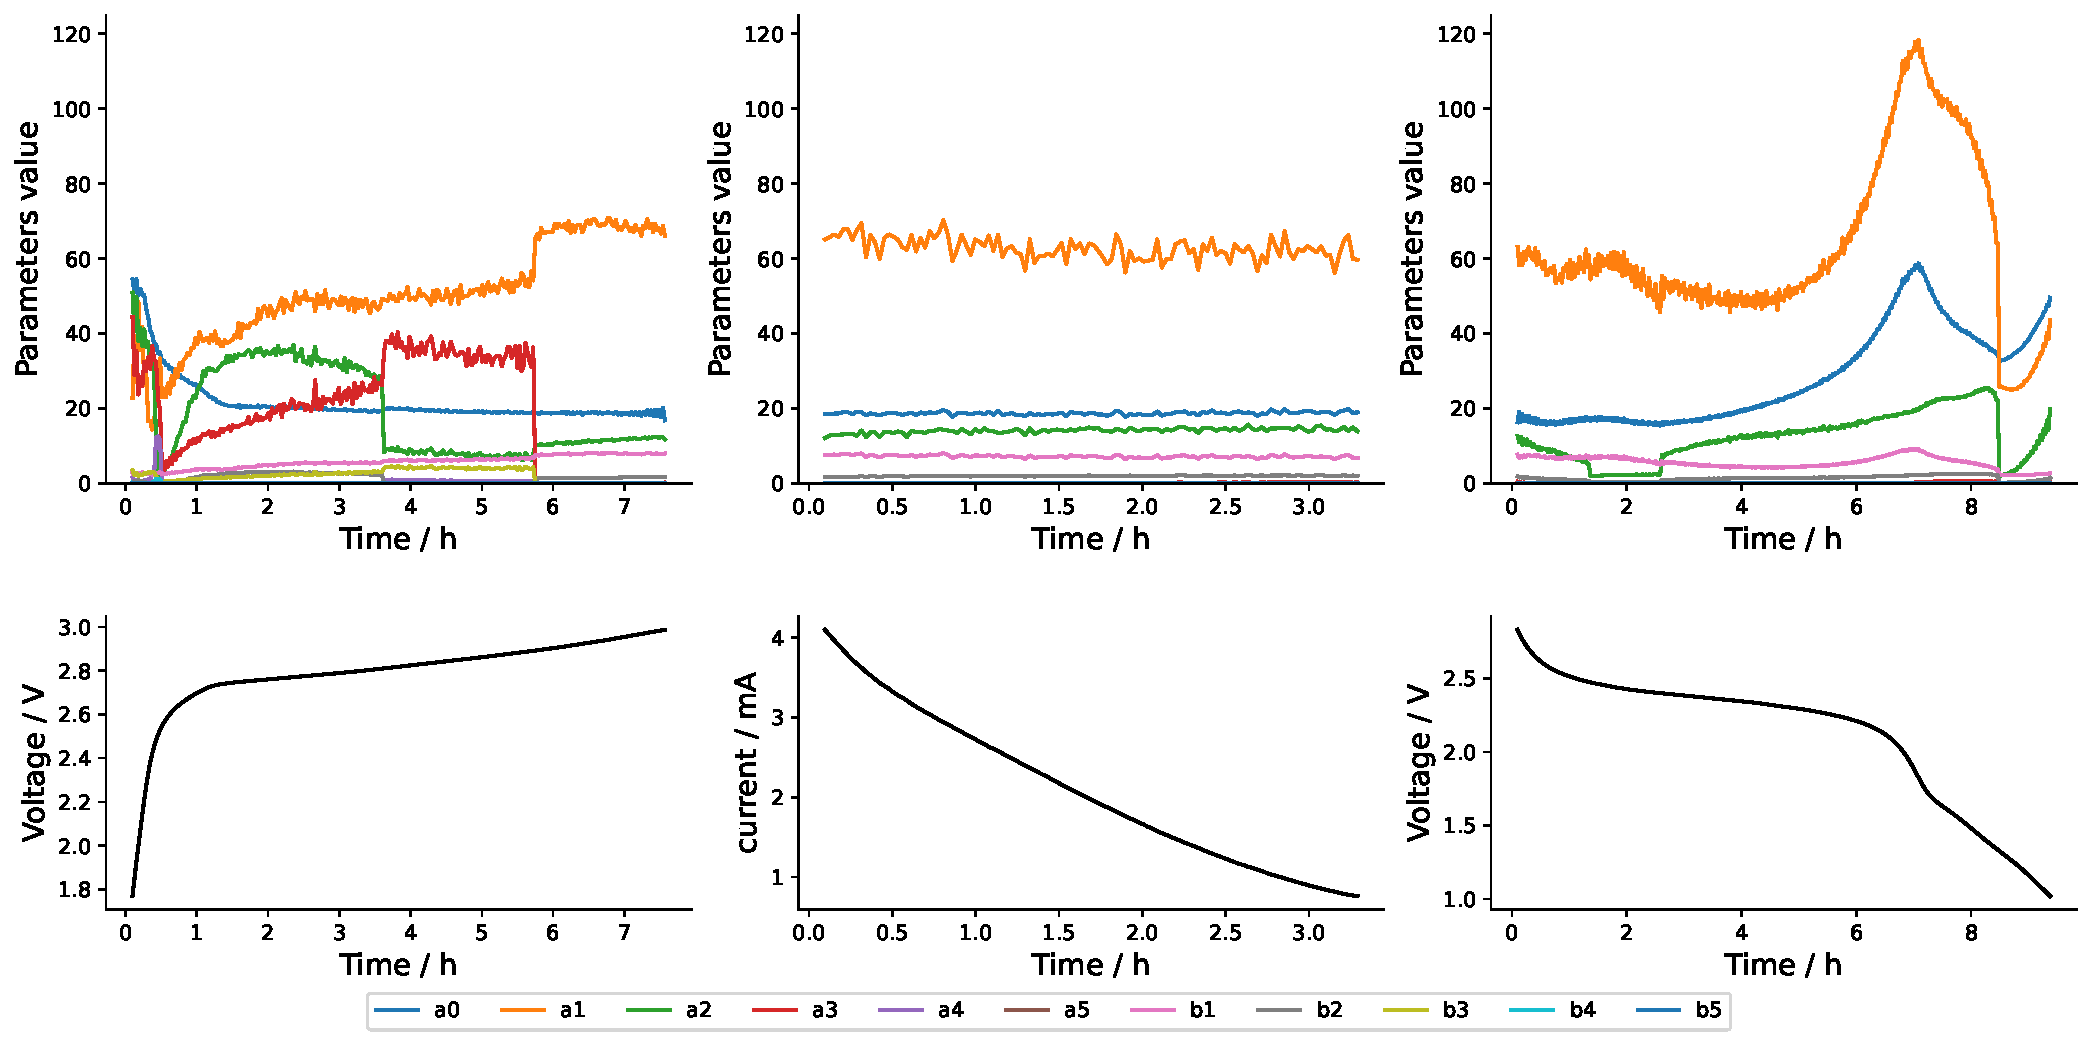
\includegraphics[width = \textwidth]{figures/results_coin/Cell009_fitting_parameters_ouput_order5_cycle4.pdf}
  \caption{Upper row: fitted rational polynomial parameters for all techniques during cycle 5.
  Lower row: corresponding cell voltage and current reconstructed via DMFA.}
  \label{fig:fitting_parameters_cycle5}
\end{figure}

\begin{figure}[!h]
  \centering
  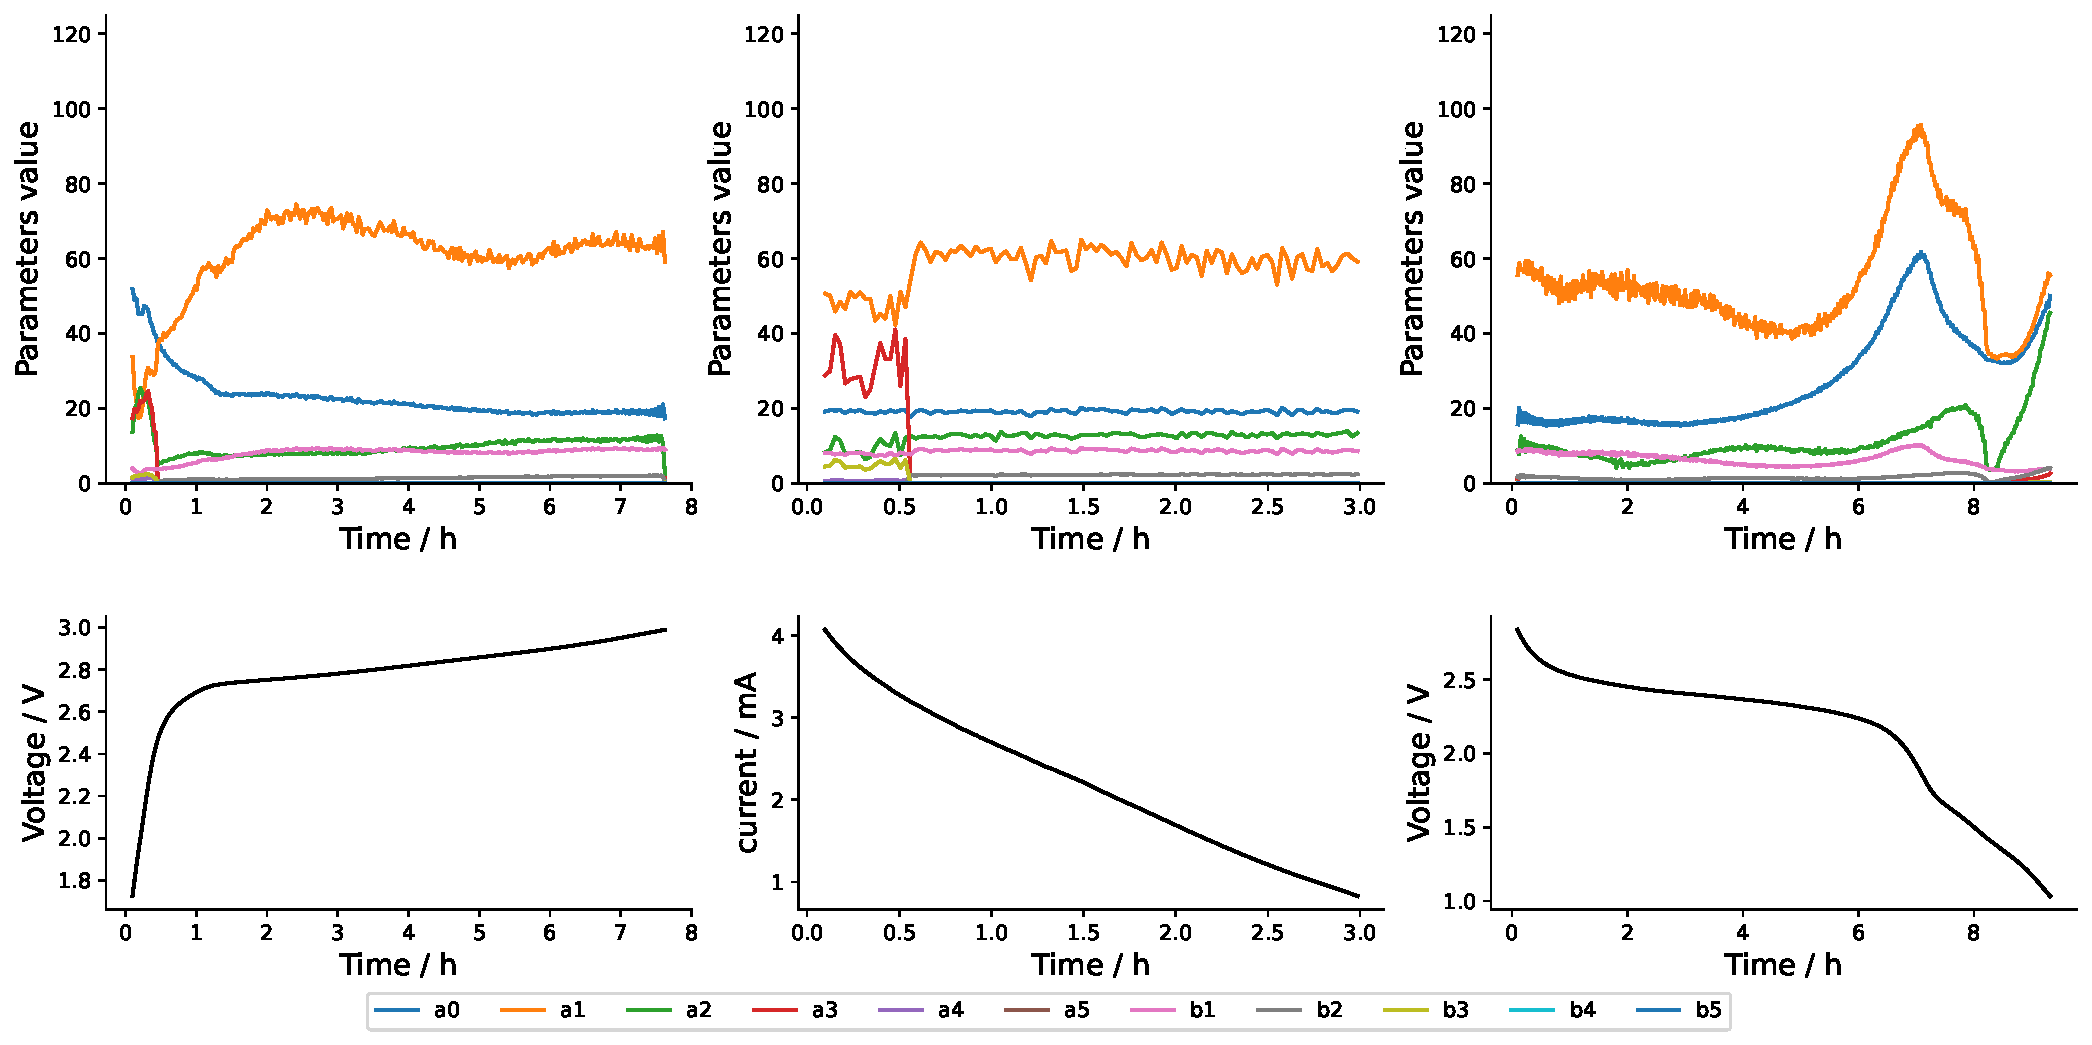
\includegraphics[width = \textwidth]{figures/results_coin/Cell009_fitting_parameters_ouput_order5_cycle9.pdf}
  \caption{Upper row: fitted rational polynomial parameters for all techniques during cycle 10.
  Lower row: corresponding cell voltage and current reconstructed via DMFA.}
  \label{fig:fitting_parameters_cycle10}
\end{figure}
\clearpage
\begin{figure}[!h]
  \centering
  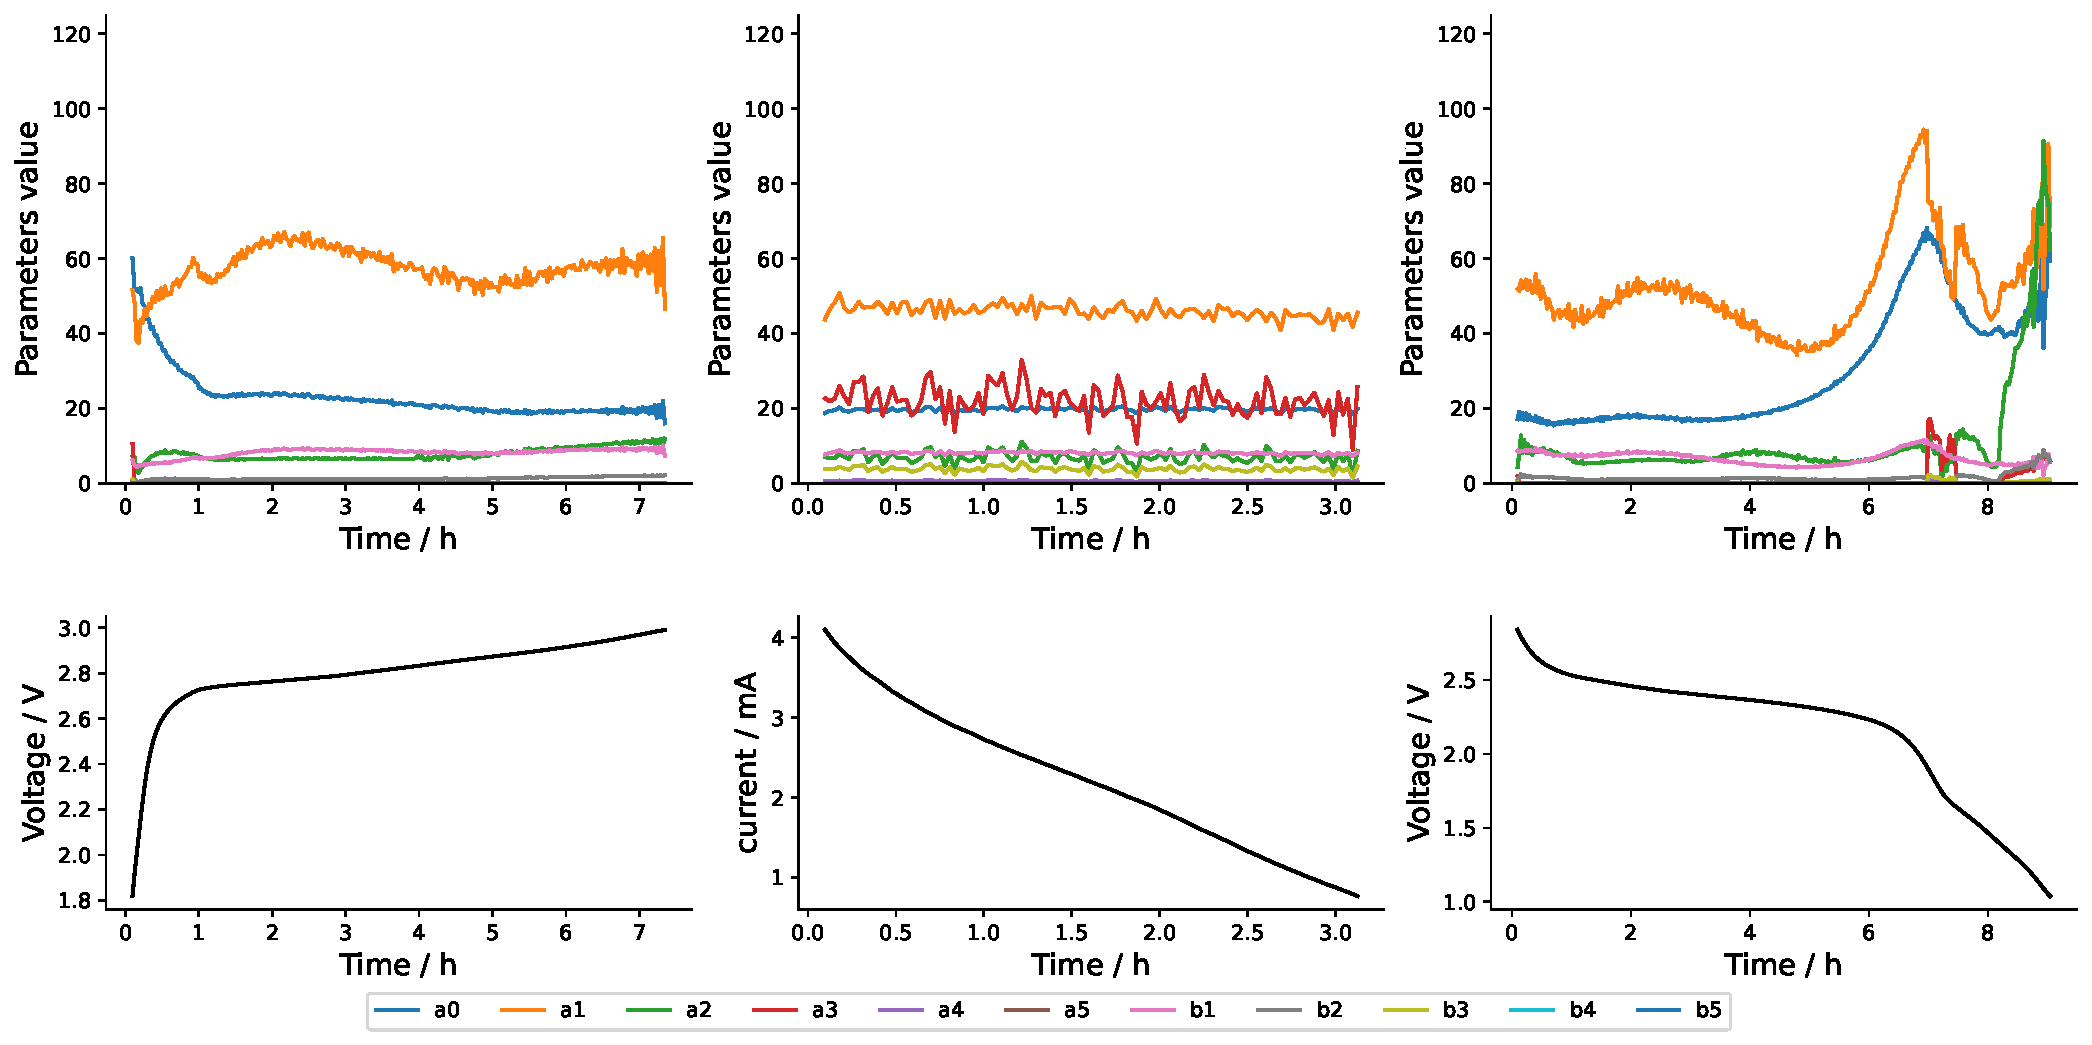
\includegraphics[width = \textwidth]{figures/results_coin/Cell009_fitting_parameters_ouput_order5_cycle14.pdf}
  \caption{Upper row: fitted rational polynomial parameters for all techniques during cycle 15.
  Lower row: corresponding cell voltage and current reconstructed via DMFA.}
  \label{fig:fitting_parameters_cycle15}
\end{figure}
\begin{figure}[!h]
  \centering
  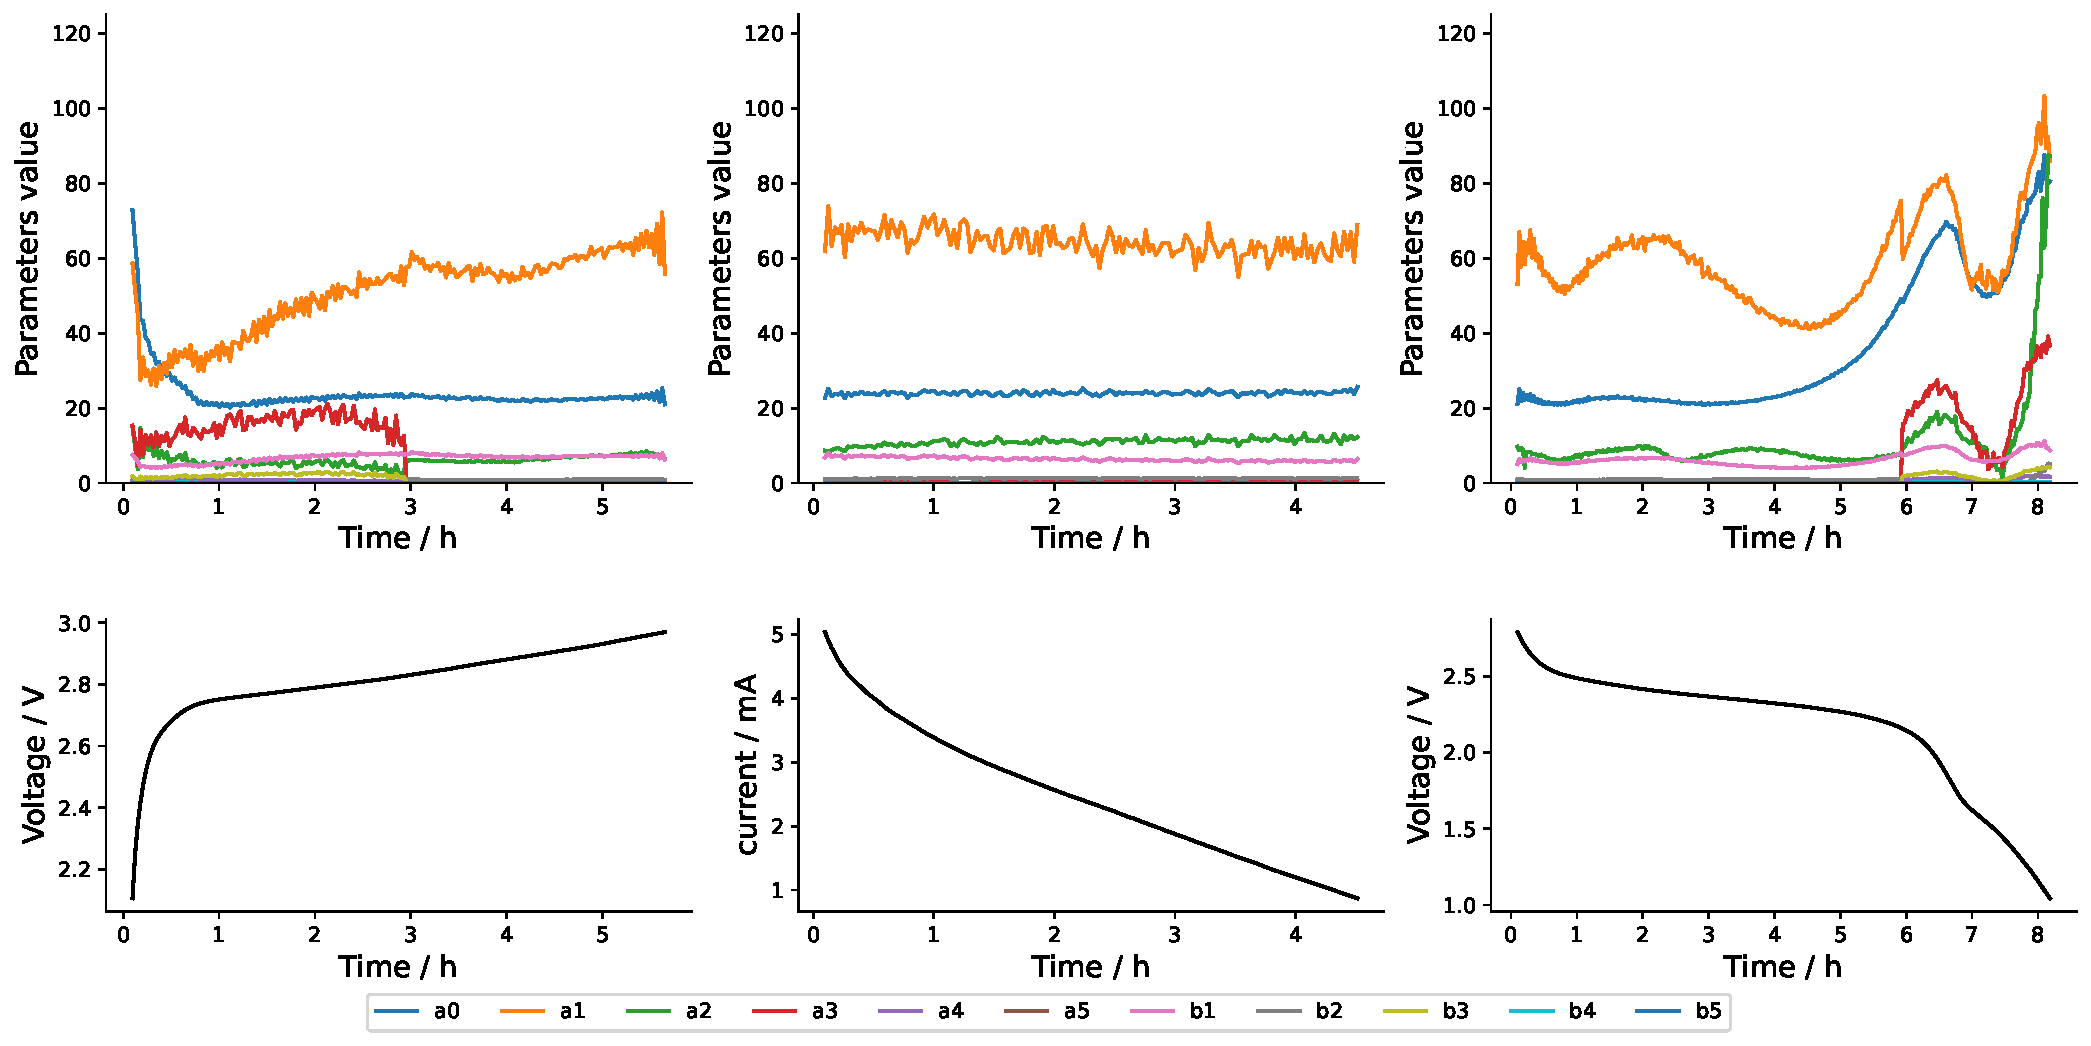
\includegraphics[width = \textwidth]{figures/results_coin/Cell009_fitting_parameters_ouput_order5_cycle19.pdf}
  \caption{Upper row: fitted rational polynomial parameters for all techniques during cycle 20.
  Lower row: corresponding cell voltage and current reconstructed via DMFA.}
  \label{fig:fitting_parameters_cycle20}
\end{figure}
\begin{figure}[!h]
  \centering
  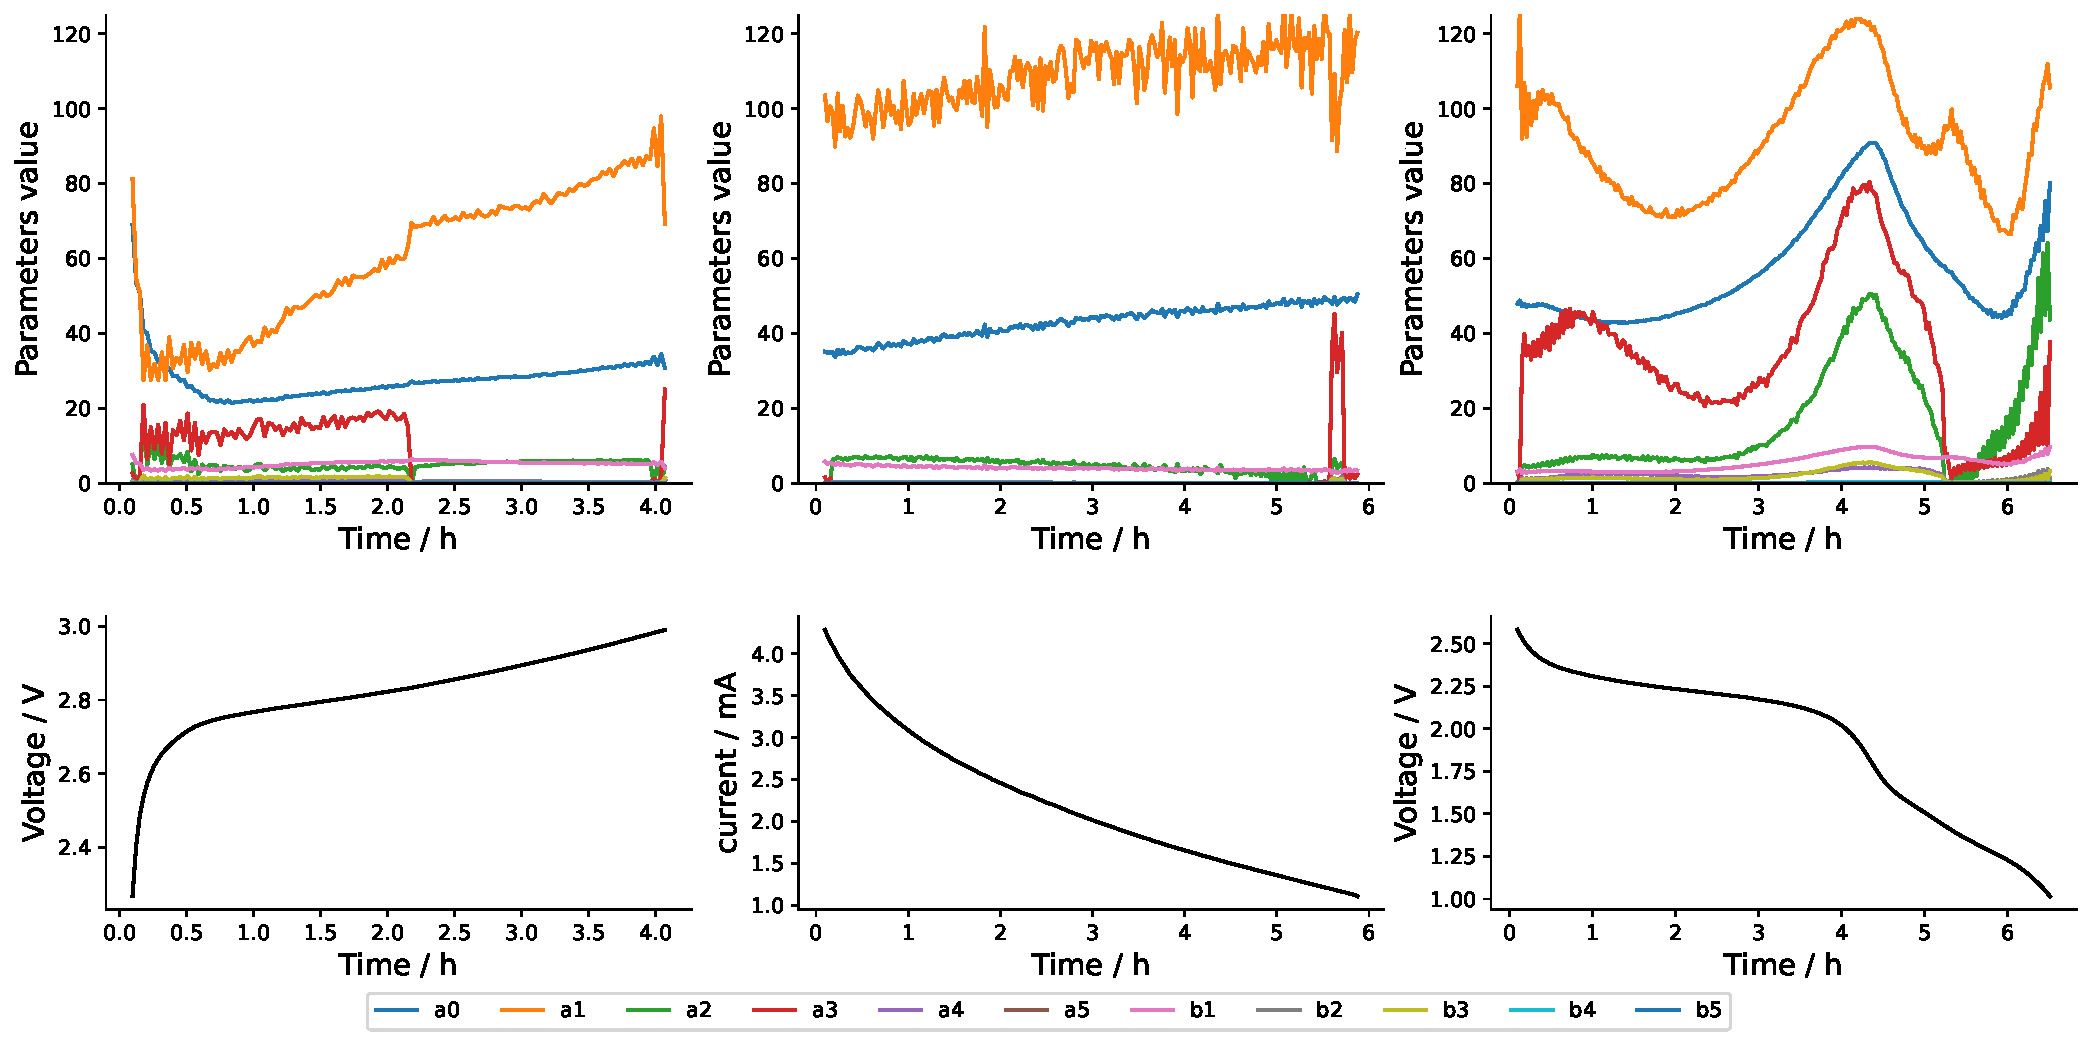
\includegraphics[width = \textwidth]{figures/results_coin/Cell009_fitting_parameters_ouput_order5_cycle21.pdf}
  \caption{Upper row: fitted rational polynomial parameters for all techniques during cycle 22.
  Lower row: corresponding cell voltage and current reconstructed via DMFA.}
  \label{fig:fitting_parameters_cycle22}
\end{figure}

However, the persistence of oscillatory residuals with increasing polynomial order, together with the systematic disparity between numerator and denominator coefficient magnitudes, reveals a structural limitation of the adopted identification formulation. 
In the least-squares estimation of rational polynomial transfer functions, the problem is \emph{ill-posed} in the sense of inverse problem theory: small perturbations in the measured impedance (e.g., noise or minor spectral features) can produce disproportionately large variations in the estimated parameters, and multiple distinct parameter sets may generate nearly indistinguishable impedance responses \cite{vogelComputationalMethodsInverse2002, ljungSystemIdentificationTheory1999}. 

This behavior is reflected in the observation that denominator coefficients often assume very small magnitudes while numerator coefficients span a significantly larger dynamic range. 
Such scaling imbalance indicates that the optimizer compensates local spectral mismatches primarily through numerator adjustments while maintaining a weakly constrained denominator structure. 
Mathematically, this corresponds to a poorly conditioned Jacobian matrix and strong correlation among parameters. 
Under these conditions, increasing the number of coefficients does not necessarily improve robustness; instead, it can lead to near pole-zero cancellations, ill-scaled parameters, and structured residuals that are not consistent with purely stochastic measurement error.
The impedance spectrum can often be reproduced accurately in magnitude, but the corresponding parameter values may not be uniquely determined or numerically stable. 
This explains why increasing model order beyond five does not eliminate oscillatory residuals and does not significantly improve parameter consistency.

Over the past three decades, alternative identification frameworks have been developed in system identification, control engineering, and RF network modeling to address precisely these issues. 
Methods such as vector fitting estimate poles and residues of rational approximations in a structured and numerically stable manner, allowing automatic determination of effective model order and reducing sensitivity to noise \cite{gustavsenRationalApproximationFrequency1999,gustavsenImprovingPoleRelocating2006}. 
Similarly, realization-based approaches such as the Loewner framework construct minimal state-space representations directly from sampled frequency data using singular value decomposition, with the model order inferred from the spectral content rather than prescribed a priori \cite{antoulasApproximationLargeScaleDynamical2005, mayoFrameworkSolutionGeneralized2007}. 
These methods do not require manual smoothing parameters and generally produce more stable dynamical representations of the impedance response, but the knowledge of industrial mathematics limits the applicability in the chemical and engineering community.
Nevertheless, the rational polynomial parametrization adopted here remains useful as a compact descriptive tool and as an initial framework for transforming complex impedance spectra into real-valued feature trajectories.

\section{Summary and implications}

In this chapter, dynamic electrochemical impedance spectroscopy was applied to commercial lithium-based coin cells operated under non-stationary charge/discharge cycling using a typical constant current--constant voltage protocol.
The objective was not to extract detailed physicochemical parameters, but to validate the proposed DEIS methodology at the full-cell level and assess its consistency, robustness, and impact on battery operation.

Continuous impedance spectra were successfully acquired throughout cycling using a broadband (7 decades) multi-sine excitation combined with online and offline signal processing.
The resulting dynamic impedance measurements capture the evolution of interfacial resistance, charge-transfer processes, and diffusion-related features as functions of both state of charge and state of health.
Comparison with classical stationary EIS measurements performed during interrupted cycling shows good agreement within the experimental variability of the cells, indicating that at moderate C-rates (C/10), the non-stationary operating conditions do not significantly alter the electrochemical state of the interfaces.

Importantly, statistical comparison of capacity retention demonstrates that continuous superimposition of the multi-sine perturbation does not affect cell aging under the investigated conditions.
This result supports the practical applicability of DEIS for long-term experiments without compromising cell integrity, at least for small-format cells and low to moderate current densities.

Dynamic impedance spectra were fitted using rational polynomial models through complex nonlinear least-squares with regularization.
Although the chosen black-box model does not provide direct physical interpretation of individual electrochemical processes, it enables real-valued parametrization of impedance evolution across cycles.
The smooth variation of fitted parameters with state of charge and state of health suggests that such representations may serve as effective features for data-driven aging diagnostics.

At the same time, the limitations of full-cell impedance analysis are evident.
The superposition of positive and negative electrode responses leads to complex models that may not be fully represented by a rational polynomial, as evidenced by oscillatory residuals.
Furthermore, a single model has limited ability to represent impedance across all operating conditions.

Nevertheless, the flexibility of rational polynomials is promising.
With proper characterization of the actual measurement error structure and systematic exploration of regularization penalty factors, the robustness of the fitting can be improved.
I suggest conducting a study with simulated electrochemical impedance data where the degrees of freedom and noise levels are known a priori.